\documentclass[12pt, a4paper]{article}

\usepackage[T1,T2A]{fontenc}
\usepackage[utf8]{inputenc}
\usepackage[english,russian]{babel}

\usepackage{pdfpages}
\usepackage{multirow}

\usepackage{caption}

\usepackage[fleqn]{amsmath}
%\usepackage{amsmath}
\usepackage{amssymb}
\usepackage{cancel}
\usepackage{xfrac}
\usepackage{tikz}
\usetikzlibrary{arrows.meta}
\usetikzlibrary{patterns}

\usepackage[hidelinks]{hyperref}

\usepackage{graphicx}
\usepackage{float}
\usepackage{wrapfig}


\setlength{\emergencystretch}{10pt}

%\usepackage{indentfirst}

\usepackage[left=2cm,right=1cm,
top=2cm,bottom=2cm,bindingoffset=0cm]{geometry}

\usepackage{setspace}
\usepackage{accents}

\usepackage{tocloft}
\setlength\cftsecnumwidth{0em}

\usepackage{titlesec}% http://ctan.org/pkg/titlesec
\titleformat{\section}%
[hang]% <shape>
{\normalfont\bfseries\Large}% <format>
{}% <label>
{0pt}% <sep>
{}% <before code>
\renewcommand{\thesection}{}% Remove section references...
\renewcommand{\thesubsection}{\arabic{section}.\arabic{subsection}}%... from subsections

\newcommand{\Int}{\int\limits}
\newcommand{\Sum}{\sum\limits}

\begin{document}

\thispagestyle{empty}

\begin{center}
	\ \vspace{-1cm}

	{Московский государственный университет имени М. В. Ломоносова}\\
	Факультет вычислительной математики и кибернетики\\
	Кафедра вычислительных методов

	\vspace{8cm}
	\begin{spacing}{2.5}
		{\huge \bfseries ВАРИАЦИОННО-ПРОЕКЦИОННЫЕ МЕТОДЫ В ЗАДАЧАХ МАТЕМАТИЧЕСКОЙ ФИЗИКИ}
	\end{spacing}


\end{center}

\vfill

\begin{center}
	Москва, 2024
\end{center}

\enlargethispage{2\baselineskip}

\newpage

\tableofcontents

\newpage

\section{Лекция 1}

\subsection{Принцип Дирихле}

Дана область $ \Omega \in \mathbb{R}^2$
\[
M = \left\{ u: \ u = u_0(x,y), \ (x,y) \in \partial \Omega \right\}
\]
Среди всех функций \( u \in M \), та функция, которая доставляет минимум <<интегралу Дирихле>> \eqref{1.1} наименьшее значение, является гармонической.
\[
\iint\limits_{\Omega}\left[{\left(\frac{\partial u}{\partial x}\right)}^2+{\left(\frac{\partial u}{\partial y}\right)}^2\right] dx dy
\tag{1.1}
\label{1.1}
\]

\subsection{Контрпример Вейерштрасса}

Наименьшее значение может и не достигаться
\[
M = \left\{ y: \ y(x) \in C'[-1;1], \ \ y(-1)=-1, y(1)=1 \right\}
\]
\[
J(y) = \int\limits^1_{-1} x^2{(y')}^2 dx, \quad J(y) \geq 0, \ \exists \inf J(y)
\]
Докажем, что нижняя граница равна нулю
\[
y_\varepsilon(x) = \frac{\arctg(\sfrac{x}{\varepsilon})}{\arctg(\sfrac{1}{\varepsilon})}
\]
\[
{y'}_{\varepsilon}(x) = \frac{1}{\arctg(\sfrac{1}{\varepsilon})} \cdot \frac{1}{1+ \frac{x^2}{\varepsilon^2}} \cdot \frac{1}{\varepsilon} = \frac{\varepsilon} {\arctg (\sfrac{1}{\varepsilon})} \cdot \frac{1}{\varepsilon^2+x^2}
\]
\[
J(y_{\varepsilon}) = \int\limits^1_{-1} x^2{(y_{\varepsilon}')}^2 dx = \int\limits_{-1}^1 \frac{x^2 \varepsilon^2}{\arctg^2(\sfrac{1}{\varepsilon})} \cdot \frac{1}{{(x^2+\varepsilon^2)}^2} dx < \frac{2 \varepsilon}{\arctg(\sfrac{1}{\varepsilon})} \xrightarrow{\varepsilon \rightarrow 0} 0
\]
\[
J(\tilde{y}) = \Int^1_{-1} x^2{(y')}^2 dx = 0 \ \Rightarrow \ y'=0 \ \Rightarrow y = \operatorname{const}
\]
Противоречие: \( y(-1)=-1, \quad y(1)=1 \)

\subsection{Контрпример Адамара}

Гармоническая функция может обращать интеграл Дирихле в бесконечность
\[
u(x,y) = \Sum_{n=1}^{\infty}\frac{{\rho^2}^{2n}}{2^n} \cos(2^n \theta); \quad x=\rho \cos \theta, \ y=\rho \sin \theta
\]
Ряд сходится в круге $\rho \leq 1$, его сумма непрерывна и гармонична внутри этого круга. Однако интеграл Дирихле этой функции, взятый по кругу $ \rho \leq r \leq 1 $ равен
\[
\pi \Sum_{n=1}^{\infty} {r^2}^{2n+1} \xrightarrow{r \rightarrow 1} \infty
\]

\subsection{Метод Ритца}
Рассмотрим функционал:
\[
J(w) = \Int_{a}^{b} f(x, w, w', \ldots, w^{(k)}) \, dx \rightarrow \inf
\]
при условии:
\[
w \in M \ \text{--- класс допустимых функций}.
\]
Используются координатные функции:
\[
\psi_0, \psi_1, \ldots, \psi_n, \ldots
\]
обладающие следующими свойствами:
\begin{enumerate}
	\item Для любого \( n \) и любых \( a_1, \ldots, a_n \in \mathbb{R} \), функция
	\[
	w_n = \psi_0 + a_1 \psi_1 + a_2 \psi_2 + \ldots + a_n \psi_n \in M.
	\]
	\item Для любого \( w \in M \) и любого \( \varepsilon > 0 \) существует \( n \in \mathbb{N} \), такое что
	\[
	\| w - \psi_0 - a_1 \psi_1 - a_2 \psi_2 - \ldots - a_n \psi_n \| < \varepsilon.
	\]
\end{enumerate}
Рассматриваем функционал
\[
J(w_n) = F(a_1, \ldots, a_n) \rightarrow \inf,
\]
удовлетворяющих уравнениям
\[
\frac{\partial J(w_n)}{\partial a_1} = 0, \quad \ldots, \quad \frac{\partial J(w_n)}{\partial a_n} = 0.
\tag{1.2}
\label{1.2}
\]
Это дает систему уравнений для определения коэффициентов \( a_1, \ldots, a_n \). \\

\textbf{Пример (задача об упругой пластине)}

Рассмотрим область \( \Omega \subset \mathbb{R}^2 \) с границей \( S = \partial \Omega \). Изгиб \( w(x, y) \) удовлетворяет уравнению Софи Жермен:
\[
\Delta^2 w = \frac{\partial^4 w}{\partial x^4} + 2 \frac{\partial^4 w}{\partial x^2 \partial y^2} + \frac{\partial^4 w}{\partial y^4} = \frac{q(x, y)}{D}, \quad (x, y) \in \Omega,
\]
где \( D \) --- жесткость пластины, \( q(x, y) \) --- интенсивность давления. \\
Краевые условия:
\[
w(x, y) = 0, \quad \frac{\partial w(x, y)}{\partial n} = 0 \quad ( \text{производная по нормали к } S).
\]
Данную задачу можно привести к следующей вариационной:
\[
J(w) = \iint\limits_{\Omega} \left[ \frac{1}{2} (\Delta w)^2 - f w \right] \, d\Omega \rightarrow \inf
\tag{1.3}
\label{1.3}
\]
где \( f \in C^{1}(\overline{\Omega}) \). \\ \\
Положим в \eqref{1.3} \( w = w_1 + w_2 \), где
\[
w_1 = - \frac{1}{8\pi} \iint\limits_{\Omega} r^2 \ln (r) f(\xi, \eta) \, d\xi \, d\eta,
\]
и \( r \) --- расстояние между точками \( (x, y) \) и \( (\xi, \eta) \in \Omega \). \\
Функционал приводится к виду
\[
J(w) = J_0 + \frac{1}{2} \iint\limits_{\Omega} (\Delta w_2)^2 \, dx \, dy \geq J_0.
\]
Таким образом, функционал \( J(w) \) ограничен снизу, а следовательно имеет точную нижнюю границу \\ \\
Введем координатные функции \( \psi_1(x, y), \psi_2(x, y), \ldots, \psi_n(x, y), \ldots \), удовлетворяющие:
\begin{enumerate}
	\item \( \psi_n(x, y) \) и их производные вида \( \frac{\partial^{k+l} \varphi_n}{\partial x^k \partial y^l} \) до порядка \( k, l \leq 3 \) принадлежат \( C(\overline{\Omega}) \)
	\item \( \psi_n(x, y) \) удовлетворяют краевым условиям
	\item Для любой функции \( \zeta(x, y) \in C^1(\Omega) \) найдется такое \(m\), что выполняется:
	\[
	|\zeta(x, y) - \sum_{i=1}^{m} a_i \psi_i(x, y)| < \varepsilon,
	\]
	а также для производных:
	\[
	\left| \frac{\partial^{k+l} \zeta}{\partial x^k \partial y^l} - \Sum_{i=1}^{m} a_i \frac{\partial^{k+l} \psi_i(x, y)}{\partial x^k \partial y^l} \right| < \varepsilon, \quad k \leq 3, l \leq 3
	\]
\end{enumerate}
Ищем приближенное решение в виде:
\[
w_n = a_1 \psi_1 + a_2 \psi_2 + \ldots + a_n \psi_n
\]
Определяем коэффициенты \( a_i \) так, чтобы \( J(w_n) \) был минимальным:
\[
J_n = \iint\limits_{\Omega} \left[ \frac{1}{2} (\Delta w_n)^2 - f w_n \right] \, dx \, dy
\]
Уравнения \eqref{1.2} в данном случае имеют вид:
\[
\Sum_{k=1}^n A_{ik} a_k = B_i, \quad i = \overline{1,n},
\tag{1.4}
\label{1.4}
\]
где
\[
A_{ik} = \iint\limits_{\Omega} \Delta \psi_i \Delta \psi_k \, dx \, dy, \quad B_i = \iint\limits_{\Omega} f \psi_i \, dx \, dy
\]
Эта система имеет единственное решение \( a_1, \ldots, a_n \), определяющее приближенное решение. \\ \\
Рассмотрим для произвольных \( b_1, b_2, \ldots, b_n \):
\[
\zeta_n = b_1 \psi_1 + b_2 \psi_2 + \ldots + b_n \psi_n
\]
Умножив уравнение \eqref{1.4} на \( b_i \) и просуммируем по всем \( i \):
\[
\Sum_{i=1}^n \Sum_{k=1}^n A_{ik} a_k b_i = \Sum_{i=1}^n B_i b_i
\]
Используя явный вид коэффициентов придем к:
\[
\iint\limits_{\Omega} (\Delta w_n \zeta_n - f \zeta_n) \, dx \, dy = 0
\tag{1.5}
\label{1.5}
\]

Решение уравнений \eqref{1.4} при подстановке в \( J_n \) доставляет ему минимальное значение (обозначим его \( J_n^{(0)} \)). Можно показать, что оно равно
\[
J_n^{(0)} = -\frac{1}{2} \iint\limits_{\Omega} (\Delta w_n)^2 \, dx \, dy
\]

С возрастанием \( n \) величина \( J_n^{(0)} \) не возрастает; в то же время она ограничена снизу. По теореме о монотонной переменной у нее есть предел. На основании критерия Коши:
\[
\forall \varepsilon >0 \quad \exists N(\varepsilon) \quad \forall n \geq N(\varepsilon) \quad \forall m: \quad 0 \leq J_n^{(0)} - J_{n+m}^{(0)} \leq \frac{1}{2} \varepsilon
\tag{1.6}
\label{1.6}
\]
Обозначим
\[
\frac{\omega_{m+n} - \omega_n}{\sqrt{\varepsilon}} = \varphi (x,y)
\]
Используя \eqref{1.5} и \eqref{1.6} с помощью некоторых преобразований можно прийти к 
\[
\iint\limits_{\Omega}{(\Delta \varphi)}^2 dx dy < 1
\]
К функции \( \varphi (x, y) \) применим формулу
\[
\varphi (x,y) = \frac{1}{2\pi}\int\limits_S \left( \varphi \frac{\partial \ln r}{\partial n} - \ln r \frac{\partial  \varphi}{\partial n} \right) dS + \frac{1}{2 \pi} \iint\limits_{\Omega} \Delta \varphi \ln r \ d\xi d \eta
\]
Поскольку \( \varphi (x, y) \) является линейной комбинацией координатных функций, она удовлетворяет граничным условиям. Получим
\[
\varphi (x,y) = \frac{1}{2 \pi} \iint\limits_{\Omega} \Delta \varphi \ln r \ d\xi d \eta
\]
Применяя неравенство Коши-Буняковского к интегралу, получим
\[
|\varphi (x,y)| \leq \frac{1}{2\pi}{ \underbrace{\left( \iint\limits_{\Omega} {(\Delta \varphi)}^2 d \xi d \eta \right)}_{\leq 1} }^{1/2} { \underbrace{\left( \iint\limits_{\Omega}{\ln}^2 r \ d\xi d\eta \right)}_{\leq C} }^{1/2}
\]
\[
|\varphi (x,y)| \leq C_1
\]
\[ |\omega_{n+m} - \omega_{n} | \leq C_1 \sqrt{\varepsilon} \]
\[ \omega_n \underset{\Omega}{\rightrightarrows}  w_n(x,y) \in C(\Omega) \]

\newpage
\section{Лекция 2}

\subsection{Метод Бубнова -- Галеркина}

Рассмотрим приближенное решение в виде:
\[
w_n = \alpha_1 \varphi_1 + \alpha_2 \varphi_2 + \ldots + \alpha_n \varphi_n + \ldots
\]
где \(L\) и \(M\) --- дифференциальные операторы, задающие задачу:
\[
L w - \lambda M w = 0
\]
Приходим к системе уравнений вида:
\[
\sum\limits_{i=1}^{n} (A_{ik} - \lambda B_{ik}) \alpha_k = 0, \quad k = \overline{1,n}
\]
Чтобы решение было ненулевым, необходимо и достаточно, чтобы определитель равнялся нулю
\[
\begin{vmatrix}
	A_{11} - \lambda B_{11} & \dots & A_{1n} - \lambda B_{1n} \\
	\vdots & \ddots & \vdots \\
	A_{n1} - \lambda B_{n1} & \dots & A_{nn} - \lambda B_{nn}
\end{vmatrix}
= 0
\]
\[
N (x,y) = L w_n - \lambda M w_n \enspace \text{--- \enspace невязка}
\]
\[
N(x,y) \perp \varphi_i, \quad i = \overline{1,n}
\]

\subsection{Повторение}

\begin{enumerate}
	\item $ f(x) \overset{\text{п.в.}}{=} 0 \Rightarrow \int\limits_{\Omega} f(x) dx = 0 $
	\item $ \int\limits_{\Omega} f(x) dx = 0, \enspace f(x) \geq 0 \enspace \Rightarrow \enspace f(x)\overset{\text{п.в.}}{=} 0 $
	\item $ |f(x)| < \varphi(x), \varphi \text{ --- суммируема по Лебегу} \Rightarrow f(x) \text{ --- суммируема по Лебегу} $
	\item $ \{\varphi_n(x)\} $ --- суммируемы с квадратами по Лебегу
	\\ \\
	$\lim\limits_{n,k \rightarrow \infty} \int\limits_{\Omega}{|\varphi_k (x) - \varphi_{n} (x)|}^2 dx = 0
	$
	\\
\end{enumerate}

Обозначим $V$ -- линейное пространство \\

$ (\varphi , \psi) - \text{скалярное произведение:} \quad (\boldsymbol{\cdot},\boldsymbol{\cdot}): V \times V \rightarrow \mathbb{C} $

\begin{enumerate}
	\item $  (\varphi, \psi) = \overline{(\psi, \varphi)} $
	\item $ (a_1 \varphi_1 + a_2 \varphi_2, \psi) = a_1 (\varphi_1, \psi) + a_2 (\varphi_2, \psi) $
	\item $ (\varphi , \varphi) \geq 0 $
	\item $ (\varphi, \varphi) = 0 \quad \Rightarrow \quad \varphi = \mathbf{0} $
\end{enumerate}

$ \| \varphi \| = \sqrt{(\varphi, \varphi)} $ \\

\begin{itemize}
	\item Неравенство Коши-Буняковского
	
	$ | (\varphi, \psi) | \leq \| \varphi \| \| \psi \|$
	
	\item Неравенство треугольника
	
	$ \| \varphi + \psi \| \leq \| \varphi \| + \| \psi \| $
\end{itemize}
\[ L_2(\Omega): \quad (\varphi, \psi) = \int\limits_{\Omega}^{} \varphi(x) \overline{\psi(x)}dx \]
\[ L_2(\Omega , \sigma): \quad (\varphi, \psi) = \int\limits_{\Omega}^{} \varphi(x) \overline{\psi(x)}\sigma (x) dx \]
\[ L_2(\Omega^m): \quad (\varphi, \varphi) = \int\limits_{\Omega}^{} \sum_{k=1}^{m} \varphi_k(x) \overline{\varphi_k(x)}dx \] \\

\textbf{Критерий линейной зависимости системы функций}

\begin{gather*}
	\varphi_1, ..., \varphi_n \text{ линейно зависима (ЛЗ) в } H
	\\
	\hspace{20mm} \Updownarrow
	\\
	\begin{vmatrix}
		(\varphi_1, \varphi_1) & \dots & (\varphi_1, \varphi_n) \\
		\vdots & \ddots & \vdots \\
		(\varphi_n, \varphi_1) & \dots & (\varphi_n, \varphi_n)
	\end{vmatrix}
	= 0
\end{gather*} \\

\textbf{Опр.} $M$ --- плотно в $H$, если $ \forall p \in H$ и $\forall \varepsilon >0 \enspace \exists \varphi_n \in M: \| \varphi_n - \varphi \| < \varepsilon $. \\

$ C_0^{(\infty)} (\Omega) $ плотно в $ L_2(\Omega) $

$\quad \quad \quad \quad \quad \uparrow$

$ \forall \varepsilon > 0 : \quad \forall \varphi \in H \quad $
\begin{tabular}[t]{l}
	$ \exists \varphi_n^1 \in C_0^{(\infty)}(\Omega) : \quad \|\varphi_n^1 - \varphi\| < \varepsilon/2 $ \\
	$ \exists \varphi_n^2 \in C_0^{\infty} (\Omega) : \quad \|\varphi_n^2 - \varphi_n^1\| < \varepsilon/2 $ \\
	$...$
\end{tabular}

$ C_0^{(k)} (\Omega) $ плотно в $ L_2(\Omega) $ \\ \\

$ \{\varphi_n \} $ --- ортонормированная система (ОНС)

$ (\varphi_n, \varphi_m) = \delta _{nm} $

$ {\|\varphi\|}^2  = {\|\varphi_1\|}^2 +{\|\varphi_2\|}^2+ ... +{\|\varphi_n\|}^2 + ...$ \\


$ \{ \varphi_n \} $ полная в  $H$, если из $ (\varphi, \varphi_k) = 0 \enspace \forall k \in \mathbb{N} \quad \Rightarrow \quad \varphi = \mathbf{0} $


$ \forall \varphi \in H: \quad a_k = (\varphi, \varphi_k) - \textrm{ коэффициенты Фурье} $ \\


\textbf{Теор.} $H$ --- гильбертово, $\{\varphi_k\}$ --- полная ортонормированная система (ПОНС) \\ \\
$ \Rightarrow {\| \varphi \|}^2 = \sum\limits^{\infty}_{k=1} {|a_k|}^2  = \sum\limits^{\infty}_{k=1} {|(\varphi, \varphi_k)|}^2 $ --- равенство Парсеваля \\ \\

\textbf{Теор.} $ \exists a_k: \quad \sum\limits_{k=1}^{\infty} {|a_k|}^2 $ сходится, $\{\varphi_n\}$ --- ПОНС в $H$, тогда: \\ \\ $\sum\limits_{k=1}^{\infty} a_k \varphi_k$ сходится по $\|\boldsymbol{\cdot}\|$ к $\varphi \in H$, при этом $\|\varphi\| = \sum\limits_{k=1}^{\infty} {|a_k|}^2$. \\ \\


\textbf{Опр.} $H$ cепарабельно если $ \exists M - $ счетное мн-во плотное в H. \\

\textbf{Теор.} $H$ сепарабельно $ \Leftrightarrow \exists $ ПОНС (счетная или конечная) в $H$. \\

$ \{ u: \int\limits_{\Omega}^{} u dx = 0 \} $ --- пример подпространства в $ L_2(\Omega) $. \\ \\

Пусть $ H_1 $ --- подпространство в $H$

$ \forall \varphi \in H \quad \exists ! \varphi_1 \in H_1: \| \varphi - \varphi_1 \| = \underset{\psi \in H_1}{\min}  \| \varphi - \psi \| $ --- проекция $\varphi$ на $H_1$

$ \varphi = \varphi_1 + \varphi_2 $, \quad \quad $ H_2 = \varphi \perp H_1 $ --- ортогональное дополнение \\

$l$ --- линейный функционал $: \quad M \subset H \rightarrow \mathbb{R}/\mathbb{C} $

$ |l_{\varphi}| \leq \|l\| \cdot {\|\varphi\|}_H $

$ \underset{\psi \rightarrow \varphi}{\lim} l_\psi = l_\varphi \quad \quad \quad \forall \varepsilon > 0 \quad \exists \delta: \| \psi - \varphi \| < \delta: \quad |l_\psi - l_\varphi| < \varepsilon$ \\ \\

\textbf{Теор. (Рисса)} $ \forall l $ --- непрерывного линейного функционала в $H$ $\exists! \psi \in H:  l_\varphi = (\varphi, \psi)$ \\ \\


Пусть $M$ --- плотно в $H$, \quad $\Phi: M \times M \rightarrow \mathbb{C} (\mathbb{R})  $

$ \Phi(\varphi, \psi): \Phi(\varphi, \psi) = \overline{\Phi(\psi, \varphi)} $

$ \Phi(\varphi, \varphi) $ --- квадратичная форма \\ \\


$ H: D_A \subset H $ --- область определения некоторого оператора А

Линейный оператор $A$ ограничен $\Leftrightarrow A$ непрерывен

$\varphi \in D_A, \quad A\varphi \in R_A$ --- область значений оператора $A$

$\varphi \in D_A \rightarrow ! \enspace A\varphi \in R_A$

\newpage
\section{Лекция 3}

\begin{equation*}
	\left.\begin{aligned}
		&Au=f \\
		&u, f \in H
	\end{aligned}\quad \right | \quad \Omega \subset \mathbb{R}^m, \quad H = L_2(\Omega)
\end{equation*}

\[
\begin{cases}
	-\Delta u = f, \qquad f \in C(\overline{\Omega}) \\
	u |_{s} = 0
\end{cases}
\]
\[ D_A = \{u \in C^2 (\overline{\Omega}); \enspace u|_s = 0\} \]
\[ A = -\Delta u \] \\

\textbf{Формула Остроградского}

\[ \int\limits_{\Omega}\left(\frac{\partial \varphi}{\partial x } + \frac{\partial \psi }{\partial y} + \frac{\partial \omega}{\partial y}\right) d\Omega = \int\limits_{S } \biggl( \varphi \cos(\overline{n} \cdot x) + \psi \cos(\overline{n}\cdot y) + \omega \cos (\overline{n} \cdot z) \biggr) dS\]
\[ W =
\begin{pmatrix}
	\varphi \\
	\psi \\
	\omega
\end{pmatrix}
\qquad \qquad \int\limits_{\Omega}^{} \text{div} W d\Omega = \int\limits_{S}^{} W_n dS
\] \\


Пусть $ \varphi = uv, \ \psi = \omega = 0 $

\[ \int\limits_{\Omega} u \frac{\partial v }{\partial x } d \Omega = - \int\limits_{\Omega}^{} v \frac{\partial u }{\partial x } d \Omega + \int\limits_{S}^{} uv \cos(\overline{n} \cdot x) dS \]

\begin{equation}
	\label{3.0}
	\tag{3.0}
	\int\limits_{\Omega } u \frac{\partial v }{\partial x_i} d \Omega = - \int\limits_{\Omega }^{} v \frac{\partial u}{\partial x_i} d \Omega + \int\limits_{S }^{} uv cos(\overline{n} \cdot x_i ) dS \qquad \text{в} \ \mathbb{R}^m
\end{equation} \\

\subsection{Формулы Грина}

\[ Lu = - \sum_{i,k =1}^{m } \frac{\partial }{\partial x_i} \left(A_{ik} (P) \frac{ \partial u(P)}{\partial x_k}\right) + C(P) u(P) \]

\[ D_L = \{ u \in C^2(\overline{\Omega}) \}, \quad P \in \Omega \subset \mathbb{R}^m, \quad C(P) \in C(\overline{\Omega}) \]
\[ A_{ik}(P) \in C(\overline{\Omega}), \quad A_{ik}(P) = A_{ki}(P) \enspace \forall P, \quad i,k=\overline{1,n} \]
\[ \int\limits_{\Omega} v Lu d \Omega = - \sum_{i,k =1}^{m }  \int\limits_{\Omega} v \frac{\partial }{\partial x_i} \left(A_{ik} \frac{ \partial u}{\partial x_k}\right) d \Omega + \int\limits_{\Omega}^{}C u v d \Omega  \]

в \eqref{3.0} подставим $ u \rightarrow v, v \rightarrow A_{ik} \frac{\partial u }{\partial x_k }$

\begin{equation}
	\label{3.1}
	\tag{3.1}
	\int\limits_{\Omega}^{} v L u d\Omega = \int\limits_{\Omega}^{} \sum_{i,k = 1}^{m}A_{ik} \frac{\partial u }{\partial x_k} \frac{\partial v }{\partial x_i} d\Omega + \int\limits_{\Omega} C u vd\Omega - \int\limits_{S }^{} v \sum_{i,k=1}^{m} A_{ik} \frac{\partial u}{\partial x_k } cos(\overline{n} \cdot x_i ) dS
\end{equation}

\begin{equation}
	\label{3.2}
	\tag{3.2}
	\int\limits_{\Omega}^{} u L u d\Omega = \int\limits_{\Omega} \left[ \sum_{i,k = 1}^{m}A_{ik} \frac{\partial u }{\partial x_i} \frac{\partial u }{\partial x_k} + Cu^2 \right] d\Omega - \int\limits_{S } u \sum_{i,k =1}^{m} A_{ik} \frac{\partial u}{\partial x_k } cos(\overline{n} \cdot x_i ) dS
\end{equation}

из \eqref{3.1} вычитаем ее же, но поменяв местами $u$ и $v$: \qquad $ \eqref{3.1} - \eqref{3.1}_{u \rightleftarrows v} $

\begin{equation*}
	\begin{split}
		\int\limits_{\Omega }^{} (vLu - uLv) d\Omega = & \int\limits_{\Omega} \cancelto{0}{\left[ \sum_{i,k = 1}^{m}A_{ik} \frac{\partial u }{\partial x_k} \frac{\partial v }{\partial x_i} - \sum_{i,k = 1}^{m}A_{ik} \frac{\partial u }{\partial x_i} \frac{\partial v }{\partial x_k} \right]} d\Omega \ - \\
		& - \int\limits_{S} \left[ v \sum_{i,k =1}^{m} A_{ik} \frac{\partial u}{\partial x_k } cos(\overline{n} \cdot x_i ) - u \sum_{i,k =1}^{m} A_{ik} \frac{\partial v}{\partial x_k } cos(\overline{n} \cdot x_k )\right] dS
	\end{split}
\end{equation*}

\[ N u := \sum_{i,k=1}^{m } A_{ik } \frac{\partial u }{\partial x_i } cos(\overline{n} \cdot x_i) \]

\begin{equation}
	\label{3.3}
	\tag{3.3}
	\int\limits_{\Omega} \left( vLu - uLv \right) d\Omega = \int\limits_{S} \left( uNv - vNu \right) dS
\end{equation}

Частный случай формул Грина, это оператор Лапласа:

\[ Lu = - \Delta u; \ A_{ii} = 1; \ A_{ik} = 0, \ i \neq k; \ C = 0 \]

\begin{equation}
	\label{3.4}
	\tag{3.4}
	- \int\limits_{\Omega} v \Delta u d\Omega  = \int\limits_{\Omega}^{} \sum_{i=1}^{m } \frac{\partial u }{\partial x_i }  \frac{\partial v }{\partial x_i} d \Omega - \int\limits_{S }^{} v \frac{\partial u }{\partial n } dS
\end{equation}

\begin{equation}
	\label{3.5}
	\tag{3.5}
	- \int\limits_{\Omega} u \Delta u d \Omega = \int\limits_{\Omega}^{} {\left(\frac{\partial u }{\partial x_i}\right)}^2 d \Omega - \int\limits_{S }^{} u \frac{\partial u }{\partial n } dS
\end{equation}

\begin{equation}
	\label{3.6}
	\tag{3.6}
	- \int\limits_{\Omega} (v \Delta u - u \Delta v ) d\Omega = \int\limits_{S }^{} \left(v \frac{\partial u }{\partial n } - u \frac{\partial v}{\partial n}\right) dS
\end{equation}

\subsection{Положительные операторы}

Пусть оператор $A$ симметричен в $H$

\textbf{Опр.} Оператор называется положительным, если $ \forall u \in D_A \subset H, \qquad (Au, u) \geq 0 \Leftrightarrow u = 0 $ \\

\textbf{Пр. 1}
\[Bu = -\frac{ d^2 }{d x^2 }u \qquad \textrm{в } L_2 (0,1); \qquad D_B = \{u \in C^2_0 (0,1): u(0) = u(1) = 0\} \]
\[ (B u, v) = - \int\limits_{0}^{1} v  \frac{d^2 u }{d x^2} dx = \int\limits_{0}^{1} \frac{du }{dx} \frac{d v }{d x } dx - v \left.\frac{d u }{dx }\right|^1_0 = - \int\limits_{0}^{1} u \frac{d^2v }{dx^2 } = (u, Bv) \quad \forall u,v \in D_B \]
\[ (Bu, u) = \int\limits_{0}^{1} {\left(\frac{du }{dx }\right)}^2 dx = 0 \]
\[ (Bu, u) = 0 \Rightarrow \frac{du }{dx } = 0 \Rightarrow u = const, u(0) = 0 \Rightarrow u = 0 \]

\textbf{Пр. 2}
\[ Cu = - \frac{ d^2 }{dx^2 }u, \qquad D_C = \left\{ u \in C^2(0,1),
\begin{cases}
	u'(0)+\alpha u(0)=0 \\
	u'(1)+\beta u(1)=0
\end{cases}
\alpha, \beta = const
\right\}
\]
\[(Cu, v) = \int\limits_{0}^{1} \frac{du}{dx} \frac{dv}{dx} dx + \alpha u(0)v(0) + \beta u(1)v(1) = (u, Cv)\]
\[\alpha > 0, \beta \geq 0\]
\[(Cu, u) = \int\limits_{0}^{1} {\left(\frac{du}{dx}\right)}^2 dx + \alpha u^2(0) + \beta u^2(1) \geq 0\]
\[\alpha = \beta = 0, \quad u \equiv 1 \Rightarrow (Cu, u) = 0 \Rightarrow C \text{ не является положительным}\]

\textbf{Пр. 3}
\[ Au = - \Delta u , \qquad D_A = \{ u \in C^2(\Omega): \quad u|_s = 0, \quad \Omega \subset \mathbb{R}^m, S = \partial \Omega, H = L_2(\Omega) \} \]
\[ (Au, u) = (-\Delta u, u ) = - \int\limits_{\Omega }^{} u \Delta u d \Omega = \int\limits_{\Omega }^{} \sum_{i = 1}^{m } {\left(\frac{\partial u }{\partial x_i }\right)}^2 d\Omega - \cancelto{0}{\int\limits_{S }^{} u \frac{\partial u }{\partial n } dS}  \geq 0 \]
\[ \frac{\partial u }{\partial x_i } = const, \ u|_s = 0 \Rightarrow u = 0 \]

\newpage

Рассмотрим мембрану

$\Omega$ в плоскости $(x,y)$, $\ u(x,y)$ --- изгиб мембраны
\[ - \Delta u = \frac{q}{T} \]

$q$ --- поперечная нагрузка на единицу площади

$T$ --- натяжение мембраны

$ {u|}_S = 0 $ --- мембрана закреплена на краях
\[ (A u , u) = (- \Delta u , u) = \iint\limits_{\Omega} \left[ \left(\frac{\partial u }{\partial x }\right)^2 + \left(\frac{ \partial u }{\partial y }\right)^2 \right] dx dy  \]

\subsection{Положительно определенные операторы}

\textbf{Опр.} Симметричный оператор $A$ называется положительно определенным, если
\begin{equation}
	\exists \gamma > 0 : (Au, u) \geq \gamma^2 {\|u\|}^2
\end{equation} \\
\textbf{Пр. 1 (продолжение)}
\[ B: u(0) = 0, u \in D_B \]
\[ u(x) = \int\limits_{0}^{x } u'(t) dt, \quad x \in [0, 1] \]
\[ u^2(x) \leq \int\limits_{0}^{x} 1^2 dt \cdot \int\limits_{0}^{x} {(u'(t))}^2 dt = x \int\limits_{0}^{x} {(u'(t))}^2 dt \leq x \int\limits_{0}^{1} {(u'(t))}^2 dt \]
\[ \int\limits_{0}^{1} u^2 (x) dx \leq \frac{1}{2} \int\limits_{0}^{1} {(u'(t))}^2 dt \]
\[ \gamma^2 \|u\|^2 \leq (Bu, u) , \quad \gamma = \sqrt{2} \quad \Rightarrow B \text{ является положительно определенным} \] \\
\textbf{Пр. 4}
\[ Lu = - \frac{d }{ d x } \left(x^3 \frac{du}{dx}\right) \quad \text{в } L_2 (0,1) \]
\[ D_L = \{u \in C^2[0,1], \ u(1) = 0 \} \]
\[(Lu, v) - (u, Lv) = \int\limits_{0}^{1} \frac{d}{dx} \left[ x^3 \left(u \frac{dv }{dx } - v \frac{du }{dx } \right)  \right] dx = \left. \left[ x^3 \left(u \frac{dv }{dx } - v \frac{du }{dx } \right) \right] \right|_0^1 = 0\]
\[ (Lu, u) = \int\limits_{0}^{1} x^3 {\left(\frac{du }{dx }\right)}^2 dx \geq 0 \quad \Rightarrow L \text{ является положительно определенным} \]
\[ \frac{(Lu, u)}{\|u\|^2} \geq \gamma^2, \qquad u_\delta (x) = \begin{cases}
	(\delta - x)^3, & 0 \leq x \leq \delta \\
	0, & \delta \leq x \leq 1
\end{cases}, \qquad u_\delta \in \mathcal{D}_L  \]
\[ \frac{(Lu_\delta , u_\delta)}{{\|u_\delta\|}^2}  = \frac{\int_{0}^{1} x^3 {(\frac{du_\delta}{dx})}^2 dx}{\int_{0}^{\delta} {(\delta -x)}^3 dx} = \frac{9 \int_{0}^{1} x^3 {(\delta -x)}^4 dx}{\int_{0}^{\delta} {(\delta -x)}^6 dx} = \frac{9}{40} \delta \quad \Rightarrow L \text{ не явл. положительно опр.} \]

\newpage

\subsection{Энергетическая норма}
Пусть $A$ --- положительно определен в $H$ (гильберт.) \\
На $D_A: \quad {[u, v]}_A = {(A u, v)}_H$ \\
Можно показать что выполняются все аксиомы скалярного произведения

\begin{enumerate}
	\item $ {[u, v]}_A = \overline{[v, u]}_A $ \\
	$ (Au, v) = (u, Av) = \overline{(Av, u)} = \overline{[v, u]} $
	\item $ [a_1 u + a_2 u, v] = a_1[u, v] + a_2[u, v]$
	\item $ (Au, u) = [u, u] \geq \gamma \|u\|^2 \geq 0 $
	\item $ [u, u] = 0 \Leftrightarrow u = 0 $
\end{enumerate}

$ |u| = [u, u] $ --- энергетическая норма

$ D_A $ предгильбертово, дополним его по $ {|\boldsymbol{\cdot}|}_A \ \Rightarrow \ $ гильбертово пр-во $ H_A $

\[ u \in H_A \Leftrightarrow \left[ \begin{array}{l}
	u \in D_A \\
	\exists u : \ \{ u_n \} \in D_A: \ | u_n - u | \underset{n \rightarrow \infty}{\rightarrow} 0
\end{array} \right. \]

\newpage
\section{Лекция 4}

\subsection{Энергетическое пространство}

Пусть $A$ --- положительно определен в $H$ (гильберт.) \\
На $D_A: \enspace \begin{array}{l}
	{[u, v]}_A = {(A u, v)}_H \\
	{\|u\|}_A = {[u,u]}_A
\end{array} $ \\
$ H_A $ --- энергетическое пространство
\[ {\|u\|}_H \leq \frac{1}{\gamma   } {\|u\|}_A \label{4.0} \tag{4.0} \]
\[ u \in H_A \begin{array}{l@{\ }l}
	\raisebox{-1ex}{$\nearrow$} & u \in D_A \\
	\raisebox{1ex}{$\searrow$} & \exists \{ u_n \} \in D_A: \ \lim\limits_{n \rightarrow \infty} {\|u_n - u\|}_A = 0
\end{array} \]


\textbf{Теор.} $ \qquad \forall u \in H_A \rightarrow $ только один элемент из $H$, причем различные $u_1, u_2 \in H_A$ отвечают различным элементам из $H$

\underline{Док-во.}

\begin{enumerate}
	\item
	$ {u_n}: \lim\limits_{n \rightarrow \infty} {\|u_n - u\|}_A = 0 $ \\
	$ {\|u_n - u_m\|}_A \leq {\|u_n - u\|}_A + {\|u_m - u\|}_A \underset{n,m \rightarrow \infty}{\rightarrow} 0 $ \\
	$ \Rightarrow {\|u_n - u_m\|}_H \rightarrow 0 $ при $ n,m \rightarrow \infty $ \\
	$ \Rightarrow \exists \lim\limits_{n \rightarrow \infty} {\|u_n - u_m\|}_H = 0 $
	
	\item
	$ u_{1, n} \underset{{\|\cdot\|}_A}{\rightarrow}  u_1, \quad u_{2, n} \underset{{\|\cdot\|}_A}{\rightarrow}  u_2 $ \\
	$ u_1 \ \text{и} \ u_2 \rightarrow u \in H, \qquad u = u_1 - u_2$ \\
	$ \exists \{u_n\} \in H_A \qquad {\|u_n - u\|}_A \rightarrow 0 $ \\
	$ \forall f \in H \qquad |(f, u_n)| \overset{\text{КБ}}{\leq} \|f\|\cdot\|u_n\| \leq {\|f\|}_A\cdot\frac{1}{\gamma}\cdot{\|u_n\|}_A \rightarrow 0 $ \\
	$ \forall \varphi \in D_A \qquad A\varphi = f \in H $ \\
	Тогда $ (A\varphi, u_n) \rightarrow 0 $ \\
	$ {[\varphi, u_n]}_A = (A\varphi, u_n) \rightarrow 0 $ \\
	Переходя к пределу: $ {[\varphi, u]}_A = 0 \ \forall \varphi \qquad \Rightarrow u = 0 \Rightarrow u_1 = u_2 \hfill \square $
\end{enumerate}

Неравенство \eqref{4.0} выполняется не только в $D_A$, но и во всем пространстве $H_A$. Пусть $u \notin D_A$, тогда:
\[ \exists \{u_n\} \in D_A \qquad {\|u_n - u\|}_A \rightarrow 0, \ \text{при этом} \ {\|u_n - u\|}_H \rightarrow 0 \]

Отсюда вытекает, что
\[ {\|u_n\|}_A \rightarrow {\|u\|}_A \qquad {\|u_n\|}_H \rightarrow {\|u\|}_H \]

Так как, $u_n \in M$, то для $u_n$ справедливо ${\|u_n\|}_H \leq \frac{1}{\gamma} {\|u_n\|}_A$. Переходя к пределу при $n \rightarrow \infty$ получим
\[ {\|u\|}_H \leq \frac{1}{\gamma} {\|u\|}_A \] \\ \\

\textbf{Пример 1}
\[ Bu = - \frac{d^2}{d x^2}u, \qquad D_{B} = \{u \in C^2 [0,1], \ u(0) = u(1) = 0 \} \]
\[ H = L_2 (0, 1), \ u \in H_B \]
\[ u \in H_B, \quad \exists \{u_n\} \in D_B \quad {\|u_n - u\|}_B \rightarrow 0 \]
\[ {\|u_n - u_k\|}_B \leq {\|u_n - u\|}_B + {\|u_k - u\|}_B \underset{n,k \rightarrow \infty}{\rightarrow} 0 \]
\[ {\|u_n - u_k\|}_B^2 = \int\limits_{0}^{1} {\left(\frac{du_n}{dx} - \frac{du_k}{dx} \right)}^2 dx \underset{n,k \rightarrow \infty}{\rightarrow} 0 \]
\[ \Rightarrow \left\{ \frac{du_n}{dx} \right\} \ \text{фундаментальна в} \ L_2(0,1) \Rightarrow \exists v(x) \in H\]
\[ u_n(x) = u_n(0) + \int\limits_{0}^{x} u_n^{'}(t) dt, \quad u_n \in D_B, \qquad \ \text{при} \ x=0:\ u_n(0) = 0 \]
\[ \text{Переходя к пределу:} \quad u(x) = \int\limits_{0}^{x} v(t) dt \quad \text{и} \quad u(0)=0\]
\[ u(1) = \int\limits_{0}^{1} v(t) dt = \lim\limits_{n \rightarrow \infty} \int\limits_{0}^{1} u_n^{'}(t) dt = \lim\limits_{n \rightarrow \infty} \left( u_n(1) - u_n(0) \right) = 0 \]
\[ \text{Следовательно,} \ u \ \text{абсолютно непрерывная на} [0,1], \text{удовлетворяет граничным условиям}\]
\[ u' \in L_2(0,1) \]

\textbf{Пример 2}
\[ Cu = - \frac{d^2}{dx^2} u(x); \qquad u'(0)+\alpha u(0)=0, \ u'(1) + \beta u(1)=0 \]
\[ \exists \{u_n\} \in D_C, \quad \alpha > 0, \ \beta \geq 0 \]
\[ \int\limits_{0}^{1} {\left( \frac{du_n}{dx} - \frac{du_k}{dx} \right)}^2 dx \underset{n, k \rightarrow \infty}{\rightarrow} 0 \]
\[ |u_n(0) - u_k(0)| \underset{n, k \rightarrow \infty}{\rightarrow} 0 \]
\[ u_n(x) = u_n(0) + \int\limits_{0}^{x} u_n'(t) dt \]
\[ u(x) = c_0 + \int\limits_{0}^{x} v(t) dt \]

\textbf{Теор.} Пусть оператор $A$ положительный, но не положительно определенный. Тогда
\[ u \in H_A: \quad u \in H \Leftrightarrow \exists \{ u_n \} \in D_A \]
\[ {\| u = u_n \|}_A \underset{n \rightarrow \infty}{\rightarrow} 0 \quad \text{и} \quad {\| u_k - u_n \|}_H \underset{n,k \rightarrow \infty}{\rightarrow} 0 \]

\textbf{Пример 3}
\[ Lu = - \frac{d}{dx} \left( x^3 \frac{du}{dx} \right), \qquad u(1)=0 \]
\[ D_L = \{u \in C^2 [0,1], \ u(1) = 0 \} \]
\[ H_L = \left\{ u \ \text{абсолютно непрерывна на} \ [0,1], \quad u(1)=0, \quad \int\limits_{0}^{1} x^3 {u'}^2 dx = 0 \right\} \]
\[ \tilde{u} = \frac{1}{x} - 1 \]

\subsection{Энергетический метод}
(для положительно определенных операторов)
\[ Au = f, \qquad A: \enspace D(A) \subset H \rightarrow H \label{4.1} \tag{4.1} \]

\textbf{Теор.} $A$ положителен в $H$, тогда уравнение \eqref{4.1} имеет не более одного решения.

\underline{Док-во.}
\[ \text{Пусть} \ u_1, u_2 \ \text{--- решения \eqref{4.1}} , \quad \tilde{u} = u_1 - u_2, \quad Au_1 = f, \quad Au_2 = f \]
\[ A \tilde{u} = 0 \]
\[ \left( A \tilde{u}, \tilde{u} \right) = {[\tilde{u}, \tilde{u}]}_A = {\| \tilde{u} \|}^2_A = 0 \hfill \square \]

\textbf{Теор. (о функционале энергии)} Если $A$ --- является положительным в $H$; $u$ --- решение уравнения \eqref{4.1} $ \Leftrightarrow $ $u$ доставляет минимум функционалу
\[ F(u) = {(Au, u)}_H - {(f, u)}_H - {(u, f)}_H \label{4.2} \tag{4.2} \]

\underline{Док-во.}

Заметим, что $D_A = D_F$ (вытекает из выражения \eqref{4.2}). Также $F(u) = (Au, u) - 2 \operatorname{Re}(u, f)$, и так как $A$ положительный оператор, то $F(u)$ принимает только вещественные значения.
\begin{itemize}
	\item[\textcircled{$\Rightarrow$}] 
	
	\[ u_0: \ Au_0 - f = 0 \]
	\[ \forall v \in D_A = D_F, \quad v = u_0 + \eta \]
	\begin{align*}
		F(v) &= (A(u_0 + \eta), u_0 = \eta) - (u_0 + \eta, f) - (f, u_0 + \eta) \overset{\text{симм.} A}{=} \\
		&= F(u_0) + (Au_0 -f, \eta) + (\eta, Au_0 - f) + (A\eta, \eta) \overset{Au_0 - f = 0}{=} \\[1ex]
		&= F(u_0) + A(\eta, \eta) \geq F(u_0) \Rightarrow u_0 = \underset{D_F}{\operatorname{argmin}} F
	\end{align*}
	
	\item[\textcircled{$\Leftarrow$}]
	
	\[ u_0 = \underset{D_F}{\operatorname{argmin}} F \]
	\[ \forall \eta \in D_A: \ v = u_0 + \lambda \eta \in D_A = D_F, \quad \lambda \in \mathbb{R} \]
	\[ F(v) \geq F(u_0) \]
	Используя симметричность $A$ приведем к виду 
	\[ 2\lambda \operatorname{Re} [(Au_0 -f, \eta)] + \lambda^2 (A\eta, \eta) \geq 0 \]
	Это возможно только тогда, когда
	\[ \operatorname{Re} [(Au_0 -f, \eta)] = 0 \]
	Заменив $\eta$ на $i \eta$, получим
	\[ \operatorname{Im} [(Au_0 -f, \eta)] = 0 \]
	Получаем
	\[ (Au_0 -f, \eta) = 0 \quad \forall u \in D_A \Rightarrow Au_0 - f = 0 \hfill \square \]
\end{itemize}

\textbf{Замеч.}
Если пространство вещественное, получим $F(u) = A(u, u) - 2(u, f)$ \\

\textbf{Пример 4}
\[ A \omega = \Delta^2 \omega = \frac{\partial^4 \omega}{\partial x^4} + 2 \frac{\partial^4 \omega }{\partial^2 x \partial^2 y} + \frac{\partial^4 \omega }{\partial y ^4} \]
\[ D_A = \left\{ \omega \in C^4(\overline{\Omega}); \quad \left. \omega \right|_S = 0; \quad \left. \frac{\partial \omega}{\partial n} \right|_S = 0 \right\} \]

\[ A \omega = \frac{q(x,y)}{\mathcal{D}} \]

\subsection{Обобщение решения задачи о min для функционала}
$A$ --- положительно определенный в $H$, $\quad Au=f \enspace \eqref{4.1}, \enspace f \in H$
\[\text{фикс.}\ f \in H \quad \forall u \in H_A \quad {(u, f)}_H: \ \text{ф-ла} \ H_A \rightarrow \mathbb{R}/ \mathbb{C} \]
\[ | {(u, f)}_H | \overset{\text{КБ}}{\leq} {\|f\|}_H {\|u\|}_H \leq {\|f\|}_H \frac{1}{\gamma} {\|u\|}_A; \qquad \gamma, \enspace {\|f\|}_H - const \qquad \Rightarrow \ \text{ограничен} \]
\[ \text{огр.} \ (f, u) \Rightarrow \ \text{по теор. Рисса} \ \exists \ u_0 \in H_A: \ {(f, u)}_H = {[u, u_0]}_A \]
\[ F(u) = {[u, u]}_A - {[u, u_0]}_A - {[u_0, u]}_A \label{4.star} \tag{4.*} \]
\[ \pm \enspace {[u_0, u_0]}_A \qquad \text{в} \ \eqref{4.star} \]
\[ F(u) = {\| u - u_0 \|}^2_A - {\|u_0\|}^2_A  \]
\[ \underset{u \in H_A}{\operatorname{argmin}} F(u) = u_0 \ \text{--- обобщенное решение} \ Au = f \] \\ \\

$H$ --- сепарабельно $\Rightarrow$ $H_A \enspace \exists \{ \omega_n \} $ ПОНС

\[ u_0 = \sum_{n=1}^{\infty} [u_0, \omega_n] \ \omega_n  \]
\[ u = \omega_n, \qquad {[u_0, \omega_n]}_A = {(f, \omega_n)}_H \]
\[ u_0 = \sum_{n=1}^{\infty} {(f, \omega_n)}_H \ \omega_n \]

\newpage
\section{Лекция 5}

\textbf{Пример} (задача о кручении стержня)

\[ \left\{ \begin{array}{l}
	-\Delta \psi = 2 G \Theta  \\
	\left. \psi \right|_{\partial\Omega} = 0  
\end{array} \right. \]

$G$ --- модуль сдвига

$\Theta$ --- угол закручивания
\[ \Omega: \left\{ \begin{array}{l}
	0 \leq x \leq a  \\
	0 \leq y \leq b  
\end{array} \right. \]
\[ Au = -\Delta u \]
\[ D_A = \left\{ u \in C^2(\Omega), \enspace \left. u \right|_{\partial \Omega} = 0 \right\} \]
\[ {[u,v]}_A = \Int_{0}^{a} \Int_{0}^{b} -\Delta v(x,y)u(x,y)dxdy \]
\[ {\| u \|}^2_A = - \Int_{0}^{a} \Int_{0}^{b} \Delta u(x,y)u(x,y)dxdy \]
\[ \psi_{m,n} = \sin \left( \frac{\pi m x}{a} \right) \sin \left( \frac{\pi n y}{b} \right) \in D_A \]
\[ \Delta \psi_{m,n} = - \pi^2 \left( \frac{m^2}{a^2} + \frac{n^2}{b^2} \right) \psi (x, y) \]
\[ {\| u \|}^2_A = \frac{\pi^2 (b^2 m^2 + a^2 n^2)}{4ab} \]
\[ w_{m,n} = \frac{2}{\pi} \frac{\sqrt{ab}}{\sqrt{b^2 m^2 + a^2 n^2}} \sin \left( \frac{\pi m x}{a} \right) \sin \left( \frac{\pi n y}{b} \right) \]
\[ (2G\Theta, w_{m,n}) = \frac{16abG\Theta}{\pi^3 m n} \sqrt{\frac{ab}{b^2 m^2 + a^2 n^2}} \]
\[ \psi(x,y) = \frac{32G\Theta a^2b^2}{\pi^4} \Sum_{m,n=1,3,5...}^{\infty} \frac{\sin \left( \frac{\pi m x}{a} \right) \sin \left( \frac{\pi n y}{b} \right)}{mn (b^2 m^2 + a^2 n^2)} \]

\subsection{Минимизация последовательностей}

$ \Phi(u) $ ограничен снизу на $M$, \quad $\exists d = \underset{u \in M}{\inf} \Phi(u)$

$ {u_n}$ --- минимизирующая, \quad $ \underset{n \rightarrow \infty}{\lim} \Phi(u_n) = d $

Пусть $u_0$ --- обобщенное решение $Au = f$

$ F(u) = {\| u - u_0 \|}_A - {\| u_0 \|}_A $

$ \underset{n \rightarrow \infty}{\lim} F(u_n) = F(u_0) = - {\| u_0 \|}_A $ \\

\textbf{Теор.} Если $A$ положительно определенный оператор в $H$, то для $\forall$ минимизирующей $\{u_n\}$ для $F(u)$:
\[ \underset{n \rightarrow \infty}{\lim} {\| u_n - u_0 \|}_A = 0 \qquad \Rightarrow {\| u_n - u_0 \|}_A \rightarrow 0 \]
\[ F(u_n) = {\| u_n - u_0 \|}_A - {\| u_0 \|}_A \rightarrow -{\| u_0 \|}_A \]

Если $u_0 \in H_A$, то теорема верна и для положительного $A$

\subsection{Расширение положительно определенного оператора}

\[ {[u,f]}_H = {[u,u_0]}_A \qquad \forall f \in H \rightarrow \exists! \ u_0 \in H_A \]
\[ \Rightarrow \text{определен линейный оператор} \ G: D_G = H \rightarrow H_A \supset R_A \qquad u_0 = Gf \]
\[ \exists \ G^{-1} \ \text{--- расширение} \ A \]

\begin{enumerate}
	\item Ограниченность
	\[ \forall u \in H_A: \enspace \left| {[u, Gf]}_A \right| \leq | {(u,f)}_H | \leq {\| f \|}_H \cdot {\| u \|}_H \leq \frac{1}{\gamma} {\| f \|}_H \cdot {\| u \|}_A \]
	\[ \text{Пусть} \ u = Gf \]
	\[ {\| Gf \|}_A^2 \leq  \frac{1}{\gamma} {\| f \|}_H \cdot {\| Gf \|}_A \]
	\[ {\| Gf \|}_A \leq  \frac{1}{\gamma} {\| f \|}_H \]
	\[ {\| Gf \|}_H \leq  \frac{1}{\gamma} {\| Gf \|}_A \]
	\[ {\| Gf \|}_H \leq  \frac{1}{\gamma^2} {\| f \|}_H \]
	\item Положительность
	\[ {(Gf,h)}_H = {[Gf, Gf]}_A = {\| Gf \|}^2_A \geq 0 \hfill \square \]
\end{enumerate}

\[ G: \ H_A \rightarrow H_A \ \ \forall f \in H_A \]
\[ {[Gf,f]}_A = {[f,GF]}_A = \overline{{(f,f)}_H} = {\| f \|}_H \geq 0 \]
\[ \text{Пусть} \ Gf = 0 \Rightarrow {(u,f)}_H = {[u, Gf]}_A = 0 \ \ \forall u \in H_A \quad \Rightarrow \quad f = 0 \]
\[ \Rightarrow G^{-1} \ \text{--- расширение} \ A \]
\[ \forall \tilde{u} \in D_A: \ G^{-1} \tilde{u} \qquad A \tilde{u} \]
\[ A \tilde{u} = f \ \Rightarrow \ \tilde{u} \ \text{--- доставляет} \ \min F(u) \]
\[ \tilde{u} = Gf, \qquad A \tilde{u} = f = G^{-1} \tilde{u} \Rightarrow G^{-1} \ \text{--- расширение} \ A \]
\[ \text{Если $A$ положительно определенный, то и $G^{-1}$ положительно определенный} \]


\subsection{Некоторые методы построения мин. последовательности}

\begin{enumerate}
	\item Процесс Ритца
	
	$H$ --- вещественное гильбертово пространство, $A$ --- положительно определенный
	\[ Au = f \]
	\[ \underset{u \in H_A}{\min} F(u) = {[u,u]}_A - 2{(u,f)}_H \]
	Введем координатные функции $ \varphi_1, \varphi_2, ..., \varphi_n, ... $
	\begin{itemize}
		\item $ \varphi_i \in H_A $
		\item $ \forall n \ {\{ \varphi_i \}}^n_{i=1} $ --- линейно независимые
		\item $ \varphi_1, \varphi_2, ..., \varphi_n, ... $ полно в $H_A$
	\end{itemize}
	\[u_n = \Sum_{k=1}^n a_k \varphi_k, \qquad a_k \in \mathbb{R} \]
	\[ F(u_n) = {\left[\Sum_{j=1}^n a_j \varphi_j, \Sum_{k=1}^n a_k \varphi_k \right]} - 2{\left(\Sum_{k=1}^n a_k \varphi_k, f \right)} = \Sum_{j,k=1}^n a_j a_k {[\varphi_j, \varphi_k]} - 2 \Sum_{k=1}^n a_k {(\varphi_k, f)} \]
	Необходимое условие: $ \min \frac{\partial F(u_n)}{\partial a_j} = 0, \ j=\overline{1,n} $. Для положительного $A$ является и достаточным условием
	\[ \frac{\partial F(u_n)}{\partial a_j} = 2 \Sum_{k=1}^n {[\varphi_j, \varphi_k]}_A a_k - 2 {(f, \varphi_j)} = 0, \qquad j=\overline{1,n} \]
	Получим СЛАУ относительно $ a_1,..., a_n $
	\[ \Sum_{k=1}^n {[\varphi_j, \varphi_k]}_A a_k = {(f, \varphi_j)} \rightarrow a_1,...,a_n \ \text{--- решение} \]
	\[ {\left( {[\varphi_k, \varphi_j]}_A \right)}_{k,j=\overline{1,n}} \ \text{--- определитель Грама} \]
	$ \exists ! $ решение $u_n = \Sum_{k=1}^n a_k \varphi_k $
	\[ \{ \varphi_n \} \rightarrow \{ w_n \} \qquad \text{ПОНС в норме} \ {\| \cdot \|}_A \]
	\[ {[w_k, w_j]}_A = \delta_{kj} \quad \Rightarrow \quad a_k = {(f, w_k)}_H = c_k \]
	\[ u_n = \Sum_{k=1}^n c_k \varphi_k \]
	\[ {\| u_n \|}^2_A = \Sum_{k=1}^n c_k^2 {(u_n, f)} = \Sum_{k=1}^n c_k^2 \]
	\[ F(u_n) = {\| u_n \|}^2_A - 2{(u_n, f)}_H = - \Sum_{k=1}^n c_k^2 = - {\| u_n \|}^2_A \]
	\[ {\| u_n \|}^2_A \leq {\| u_0 \|}^2_A, \qquad {\| u_n \|}^2_A \underset{n \rightarrow \infty}{\rightarrow} {\| u_0 \|}^2_A \]
	\[ \text{Пусть} \ n>k: \ {\| u_n - u_k \|}^2_A = {\left\lVert \Sum_{i=k+1}^n c_i w_i \right\rVert}^2_A = \Sum_{i=k+1}^n c_i^2 = {\| u_0 \|}^2_A - {\| u_k \|}^2_A \]
	\[ \forall u \in H_A, \qquad w_1 = \frac{u}{{\| u \|}_A} \]
	\[ n = 1, \qquad u_1 = c_1 w_1, \quad c_1 = {(f, w_1)}_H \]
	\[ {\| u_0 \|}^2_A \geq {\| u_1 \|}^2_A = c_1^2 = {({(f, w_1)}_H)}^2 = {({(f, u_1)}_H)}^2 \cdot \frac{1}{{\| u_1 \|}^2_A} \]
	\[ {\| u_0 \|}^2_A \geq \frac{{({(f, u)}_H)}^2}{{\| u \|}^2_A} \quad \forall u \in H_A \]
	
	\item Метод Куранта
	\[ Au = f, \qquad \Omega \subset \mathbb{R}^m + \ \text{граничные условия} \ \partial \Omega  \]
	\[ \Phi (u) = F(u) + \underbrace{\Sum_{j=0}^k \Sum_{\alpha_1 + ... + \alpha_n = j} {\left\lVert \frac{\partial^j (Au - f)}{{\partial x_1}^{\alpha_1} \cdot ... \cdot {\partial x_n}^{\alpha_n}} \right\rVert}_H^2}_{\geq 0}, \qquad f \in C^k(\Omega) \]
	\[ \Phi (u) \geq F(u) \]
	\[ u_0 = \underset{H_A}{\operatorname{argmin}} \ F(u) \]
	\[ \{ u_n \} \ \text{--- минимизирует} \ \Phi(u) \]
	
	\textbf{Пример}
	\[ -\Delta u = f, \quad u|_{\partial \Omega} = 0, \quad \Omega \subset \mathbb{R}^2 \]
	Положим $k = 0$
	\[ \Phi(u) = {(-\Delta u, u)}_H - 2 {(u, f)}_H + {\| \Delta u + f \|}_H^2 \]
	\[ \Phi(u) = \Int_\Omega {\left\{ {\left(\frac{\partial u}{\partial x}\right)}^2 + {\left(\frac{\partial u}{\partial y}\right)}^2 - 2uf + {(\Delta u + f)}^2 \right\}} d\Omega \]
	\[ \{ u_n \} \ \text{--- минимизирующая для } \Phi, \qquad \Int_{\Omega} {(\Delta u_n + f)}^2 d \Omega \rightarrow 0 \]
	\[ u_n(x, y) - u(x, y) = - \Int_{\Omega} G(x, y; \xi, \eta) (\Delta u_n + f) d \Omega \]
	\[ | u_n(x, y) - u(x, y) | \leq \sqrt{\Int_{\Omega} G^2(x, y; \xi, \eta) d \xi d \eta} \sqrt{\Int_{\Omega} {(\Delta u + f)}^2 d \Omega } \]
	\[ | u_n(x, y) - u(x, y) | \leq C \sqrt{\Int_{\Omega} {(\Delta u + f)}^2 d \Omega } \]
	\[ \{ u_n \} \overset{\Omega}{\rightrightarrows} u(x, y) \]
	
	\item Метод наискорейшего спуска
	\[ Au = f \]
	\[ m {\| u \|}^2_H \leq {(Au, u)}_H \leq M {\| u \|}^2_H \]
	\[ F(u) = {(Au, u)}_H - 2{(u,f)}_H \]
	
	\raisebox{.5pt}{\textcircled{\raisebox{-.9pt} {1}}} $ \quad \forall u_1: \qquad v_1 = Au_1 - f, \qquad u_2 = u_1 - a_1 v_1 $
	\[ F(u_1 - a_1v_1) = F(u_1) - 2a_1 \Bigl[ {(Au_1, v_1)}_H - {(f,v_1)}_H \Bigr] + a_1^2 {(Av_1, v_1)}_H \]
	\[ a_1 {(Av_1, v_1)}_H - \Bigl[ {(Au_1, v_1)}_H - {(f,v_1)}_H \Bigr] = 0 \]
	\[ {(Au_1, v_1)}_H - {(f,v_1)}_H = {(Au_1 - f, v_1)}_H = {(v_1, v_1)}_H = {\| v_1 \|}^2_H \]
	\[ a_1 = \frac{{\| v_1 \|}^2_H}{{(Av_1, v_1)}_H} \]
	\raisebox{.5pt}{\textcircled{\raisebox{-.9pt} {2}}} $ \quad \forall u_2: \qquad v_2 = Au_2 - f_1, \qquad u_3 = u_2 - a_2 v_2 $
	\[ ... \]
	\raisebox{.5pt}{\textcircled{\raisebox{-.9pt} {n}}} $ \quad {\| u_{n+1} - u_0 \|}_A \leq {\| u_1 - u_0 \|}_A {\Bigl(\frac{M-m}{M+m}\Bigr)}^n $
	
\end{enumerate}

\subsection{Краевые задачи для ОДУ}

\[ Lu = - \frac{d}{dx} \left( \Phi(x) \frac{du}{dx} \right) + q(x)u'(x) \]
\[ Lu = f(x), \qquad x_1 < x \leq x_2 \]
\[ \left\{ \begin{array}{l}
	\alpha_1 u'(x_1) + \beta_1 u(x_1) = 0 \\
	\alpha_2 u'(x_2) + \beta_2 u(x_2) = 0
\end{array} \right. \]
\[ D_L = \{ C^2[x_1, x_2] + \ \text{граничные условия} \} \]
Пусть
\begin{itemize}
	\item $ p(x) \geq 0, \enspace q(x) \geq 0, \quad x \in [x_1, x_2] $ \\ ($p$ может обращаться в 0 в некоторых точках) $ p(x) \geq p_0 > 0 $
	\item $ p \in C^1[x_1, x_2], q \in C[x_1, x_2] $
	\item $ \Int_{x_1}^{x_2} \frac{dx}{p(x)} $ сходится на $ [x_1, x_2] $
	\item $ \alpha_i^2 + \beta_i^2 > 0, \quad i = 1, 2 $
\end{itemize}
\[ (Lu, v) = \Int_{x_1}^{x_2} \left[ p(x) \frac{du}{dx} \frac{dv}{dx} + q(x) u(x) v(x) \right] dx + \frac{\beta_1}{\alpha_1} p(x_1) u(x_1) v(x_1) + \frac{\beta_2}{\alpha_2} p(x_2) u(x_2) v(x_2) \]
\[ (Lu, u) = \Int_{x_1}^{x_2} \left[ p(x) {\left(\frac{du}{dx}\right)}^2 + q(x) u^2(x) \right] dx + \frac{\beta_1}{\alpha_1} p(x_1) u^2(x_1) + \frac{\beta_2}{\alpha_2} p(x_2) u^2(x_2)  \]
\[  \blacktriangleright \alpha_1 = \alpha_2 = 0 \]
\[ (Lu, u) \geq p_0 \Int_{x_1}^{x_2} \left[ p(x) {\left(\frac{du}{dx}\right)}^2 \right] dx = p_0 {\| u' \|}^2_H \geq \gamma^2 {\| u \|}^2_H, \qquad \gamma = \frac{\sqrt{2p_0}}{x_2 - x_1} \]
\[ u(x_1)=0 \ \rightarrow \ u(x) = \Int_{x_1}^{x} u'(t) dt \]
\[ u^2(x) \leq (x_2 - x_1) {\| u' \|}^2_H \]
\[ \Int_{x_1}^{x_2} (...) \ dx \quad \Rightarrow \quad {\| u \|}^2_H \leq \frac{x_2 - x_1}{2} {\| u' \|}^2_H \]
\[ \blacktriangleright \beta_1 > 0 \]
\[ (Lu, u) \geq \frac{B}{C} {\| u \|}^2_H \]
\[ C = \max\left\{2A(x_2 -x_1), 2(x_2 - x_1)\right\}, \quad B = \min\left\{\frac{\beta_1}{\alpha_1} p(x_1), 1\right\} \]
\begin{multline*}
	F(u) = {(Lu, u)}_H - 2{(u,f)}_H = \frac{\beta_1}{\alpha_1} p(x_1) u^2(x_1) + \frac{\beta_2}{\alpha_2} p(x_2) u^2(x_2) + \\ + \Int_{x_1}^{x_2} \left[ p(x) {u'(x)}^2 + q(x) u^2(x) - 2f(x)u(x) \right] dx
\end{multline*}
\[ u_n(x) \underset{{\| \cdot \|}_A}{\rightarrow} u_0(x) \]
\[ \underset{n \rightarrow \infty}{\lim} {\| u_n - u_0 \|}_A = 0, \qquad {\| u_n - u_m \|}_A^2 \rightarrow 0 \]
\[ \underset{n,m \rightarrow \infty}{\lim} \left[ u_n(x) - u_m(x) \right] = 0 \]
\[ \underset{n,m \rightarrow \infty}{\lim} \Int_{x_1}^{x_2} {\left[ {u'}_n(x) - {u'}_m(x) \right]}^2 dx = 0 \]
\[ u_n(x) - u_m(x) = u_n(x_1) - u_m(x_1) - \Int_{x_1}^{x_2} {\left[ {u'}_n(t) - {u'}_m(t) \right]}^2 dt \]
Используя неравенство Буняковского и $ {a+b}^2 \leq a^2 + b^2 $
\[ {| u_n(x) - u_m(x) |}^2 \leq 2 {(u_n(x_1) - u_m(x_1))}^2 + 2(x_2 - x_1) \Int_{x_1}^{x_2} {\left[ {u'}_n(t) - {u'}_m(t) \right]}^2 dt \]
\[ u_n(x) \rightrightarrows u(x) \]
\[ {u'}_n \overset{\text{ср}}{\rightarrow} u'(x) \]

\newpage
\section{Лекция 6}

\subsection{Применение энергетического метода для краевых задач}

\textbf{Пример 1}

\[ Lu =\Sum_{k=0}^m (-1)^k \frac{d^k}{{dx}^k} \left[ p_k(x) \frac{d^k u}{{dx}^k} \right], \qquad Lu = f \]
\[ \left\{ \begin{array}{l}
	u(x_1) = u'(x_1) = ... = u^{(m-1)}(x_1) = 0 \\ 
	u(x_2) = u'(x_2) = ... = u^{(m-1)}(x_2) = 0
\end{array} \right. \]
\[ p_k(x) \geq 0, \quad x \in [x_1, x_2], \qquad f \in L_2(x_1, x_2) \]
\[ D_L = \left\{ u \in C^{2m}[x_1, x_2] + \ \text{граничные условия} \right\} \]
\[ {(Lu, u)}_H = \Sum_{k=0}^{m} \Int_{x_1}^{x_2} p_k (x) {\left(\frac{d^k u }{{dx}^k }\right)}^2 dx \geq \Int_{x_1}^{x_2} p_m (x) {\left(\frac{d^m u }{{dx}^m }\right)}^2 dx \geq p_0 \Int_{x_1}^{x_2} {\left(\frac{d^m u }{{dx}^m }\right)}^2 dx = p_0 {\|u^{(m)}\|}^2_H \]

Так как выполняется $ u(x_1) = u'(x_1) = ... = u^{(m-1)}(x_1) = 0 $, то
\[ {\| u \|}_H^2 \leq \frac{{(x_2-x_1)}^2}{2} {\| u' \|}_H^2 \]
\[ {\| u \|}_H \leq \frac{x_2 - x_1}{\sqrt{2}} {\| u' \|}_H, \ \ ..., \ \ {\| u^{(l-1)} \|}_H \leq \frac{x_2 - x_1}{\sqrt{2}} {\| u^{(l)} \|}_H, \qquad l=\overline{1,m} \]
\[ {\| u^{(m)} \|}_H^2 \geq {\left(\frac{\sqrt{2}}{x_2 - x_1}\right)}^m {\| u \|}_H^2 \]
\[ (L u_m ) \geq \gamma^2 {\|u\|}^2_H, \quad \gamma = \sqrt{p_0} {\left(\frac{\sqrt{2}}{x_2-x_1}\right)}^m \qquad \Rightarrow \qquad L \ \text{--- положительно определенный} \]
\[ {\|u\|}_A \leq \sqrt{p_0} \ {\| u^{(m)} \|}_H, \quad \exists \ \{ u_n (x) \}\]
\[ \underset{n \rightarrow \infty}{\lim} {\| u_n - u_0 \|} = 0, \quad u_0 \ \textrm{--- точное решение} \]
\[ {\|u_n - u_k \|}_A \leq {\|u_n - u_0\|}_A + {\| u_k - u_0\|}_A \rightarrow 0 \]
\[ u^{(l)}_n (x_1) = u^{(l)}_k (x_1) = 0, \quad l = \overline{0, m-1} \]
\[ u^{(m - 1)}_n (x) - u^{(m - 1)}_k (x) = \Int_{x_1}^{x} \left( u^{(m)}_n (t) - u^{(m)}_k (t) \right) \ dt \]
\begin{multline*}
	\left| u^{(m - 1)}_n (x) - u^{(m - 1)}_k (x) \right| \overset{\text{КБ}}{\leq} (x - x_1) \Int_{x_1}^{x} {\left( u^{(m)}_n (t) - u^{(m)}_k (t) \right)}^2 \ dt \leq \\
	\leq (x_2 - x_1) \Int_{x_1}^{x_2} {\left( u^{(m)}_n (t) - u^{(m)}_k (t) \right)}^2 \ dt \leq (x_2 - x_1) {\left\| u^{(m)}_n - u^{(m)}_k \right\|}_H^2
\end{multline*}

\textbf{Пример 2} (задача об изгибе балки)
\[ L\omega = \frac{d^2}{{dx}^2} \left[E I(x) \frac{d^2 \omega }{{dx}^2}\right] + K\omega = q(x)\]

$ \omega $ --- прогиб балки

$ E $ --- модуль Юнга

$ I(x) $ --- момент инерции сечения

$ q(x) $ --- интенсивность нагрузки на балку

$ K $ --- коэффициент податливости основания
\[ \omega (0) = \omega (l) = 0 \]
\[ \omega'(0) = \omega'(l) = 0 \]

Из предыдущей задачи известно, что $L$ положительно определен
\[ F(\omega) = \Int_{0}^{l} \left(E I(x) {\omega''}^2 + K\omega^2 - 2q(x) \omega \right) dx = (L\omega , \omega) -2 (\omega, q)\]

Воспользуемся методом Ритца
\[ {\{\varphi_n (x)\}}^{\infty}_{n=1}, \quad \varphi_n (x) = {(x-l)}^2 x^{n+1}, \quad \text{полная система в} \ H_A \]
\[ \omega_n = \Sum_{k=1}^{n} a_k \varphi_k (x) = {(x-l)}^2 \Sum_{k=1}^{n} a_k x^{k+1} \]
\[ \Sum_{k=1}^{n} a_k A_{ik} = b_{ij}, \quad i=\overline{1, n} \]
\[ b_j = {(q, \varphi_j)}_H = \Int_{0}^{l } q(x) {(x-l)}^2 x^{j+1} dx \]
\[ A_{ik} = {(L \varphi_i, \varphi_k)}_H = \Int_{0}^{l} \left(E I(x) \frac{d^2 \varphi_i}{{dx}^2} \frac{d^2 \varphi_k}{{dx}^2} + k\varphi_i \varphi_k \right) dx \]
\[ \omega_n(x) \underset{[0;l]}{\rightrightarrows} w_0(x), \qquad {\omega'}_n(x) \underset{[0;l]}{\rightrightarrows} {w'}_0(x), \qquad {\omega''}_n(x) \overset{\text{ср}}{\rightrightarrows} {w''}_0(x), \]
\[ \omega(0) = 0, \qquad \omega''(l) = 0, \qquad \omega' (0) = 0 \]
\[ {\left.{\frac{d}{dx} \left(E I(x) \frac{d^2 \omega }{d x^2}\right)}\right|}^{x=l}_{x=0} = 0 \]

\textbf{Пример 3} (краевая задача для систем ОДУ)
\[ - \Sum_{k=1}^{s} \left[ \frac{d}{dx} \left( p_{jk}(x) \frac{du_k (x)}{dx} \right) - q_{jk}(x) u_k (x) \right] = f_j(x) \]
\[ u_j(x_1) = u_j(x_2) = 0 \]
\[ u(x) = {\bigl(u_1(x), ..., u_j(x)\bigr)}^T, \qquad f(x) = {\bigl(f_1(x), ..., f_j(x)\bigr)}^T \]
\[ {\bigl( p_{jk}(x) \bigr)}_{j,k=1} \subset P(x), \qquad {\bigl( q_{jk}(x) \bigr)}_{j,k=1} \subset Q(x) \]
\[ - \frac{d}{dx} \left[P(x) \frac{du}{dx} \right] + Q(x) u(x) = f(x) \]
\[ u(x_1) = u (x_2) = 0 \]
\[ p_{jk}(x), \ q_{jk}(x), \ {p'}_{jk} (x) \in C[x_1, x_2] \]
\[ {(u, v)}_{H= L_2(x_1, x_2)} = \Int_{x_1}^{x_2} u (x) v(x) dx = \Int_{x_1}^{x_2} \Sum_{k=1}^{s} u_k(x) v_k (x) dx \]
\[ D_A = \left\{ u = {\bigl(u_1, ..., u_j\bigr)}^T, \ u_i(x) \in C[x_1, x_2], \ u_i(x_1) = u_i(x_2) = 0 \right\} \]

\textbf{Теор.} $P(x), Q(x)$ симметричны на $ x \in [x_1, x_2] \quad \Rightarrow \quad A $ симметричный

\underline{Док-во.}
\begin{multline*}
	{(Au, v)}_H = - \Int_{x_1}^{x_2} v(x) \frac{d}{dx} \left[P(x) \frac{du}{dx}\right] dx \ + \Int_{x_1}^{x_2} v(x)  Q(x) u(x) dx = \\
	= \Int_{x_1}^{x_2} \left[P \frac{du }{dx } \frac{dv}{dx} + v(x) Q(x) u(x) \right] dx = {(u, Av)}_H \quad \Rightarrow \quad \text{симметр.}
\end{multline*}
\[ Q u v = \Sum_{j,k=1}^{s } q_{jk} u_k v_j = \Sum_{i,j =1}^{s} q_{kj} v_j u_k \hfill \square \]

\textbf{Теор.} $P(x), Q(x)$ симметричны на $[x_1, x_2]$, $P(x)$ --- полож. опр.,  $Q(x)$ неотр. на $[x_1, x_2] \Rightarrow A $ положительно определен

\underline{Док-во.}
\[ P(x) \textrm{ пол. опр } \forall x \Rightarrow \textrm{ пусть } \lambda_1(x) >0  \]
\[ \exists \ \tilde{\lambda} > 0 = const, \quad \lambda_1(x) > \tilde{\lambda} > 0, \quad  x \in [x_1, x_2] \]
\[ \forall \ t = {\bigl(t_1, ..., t_s\bigr)}^T \]
\[ P(x) t \cdot t = \Sum_{j, k=1}^{s } P_{jk}(x)t_j t_k \geq  \lambda_1(x) \Sum_{k=1}^{s } t_k^2 \geq \tilde{\lambda } \Sum_{k=1}^{s } t^2_k \]
\[ Q(x) t\cdot t = \Sum_{j, k=1}^{s }q_{jk} t_j t_k \geq 0 \]
\[ {(Au, u)}_H = \Int_{x_1}^{x_2} \left(P \frac{du }{dx } \cdot \frac{du }{dx} + Qu \cdot u \right) dx \geq \tilde{\lambda } \Int_{x_1}^{x_2} \Sum_{k=1}^s {\left(\frac{du_k}{dx}\right)}^2 dx \]
\[ (Au, u)_H \geq \frac{2 \tilde{\lambda}}{{(x_2 - x_1)}^2} \Int_{x_1}^{x_2} \left(\Sum_{k=1}^{s } u_k^2\right) dx = \frac{2 \tilde{\lambda}}{{(x_2 - x_1)}^2} {\|u\|}^2_H \]
\[ {(Au, u)}_H \geq \gamma^2 {\|u\|}^2_H \hfill \square \]


\[ \left. \begin{array}{l}
	u'(x_1) - M_1 u(x_1) = 0 \\
	u'(x_2) - M_2 u(x_2) = 0
\end{array} \right. \quad \Rightarrow \quad A \ \text{--- полож. опр.}, \quad M_1, M_2 \ \text{--- ?? неотриц.} \]

\subsection{Основные краевые задачи для ур-я Пуассона}

\[ -\Delta u = f(p) \qquad \text{в} \ \ \Omega \subset \mathbb{R}^m \label{6.1} \tag{6.1} \]

$ \blacktriangleright $ \underline{задача Дирихле}
\[ u|_{\partial \Omega} = 0 \label{6.2} \tag{6.2}  \]
\[ A u = - \Delta u = - \Sum_{k=1}^{m } \frac{\partial^2 u }{\partial {x_k}^2} \]
\[ D_A = \left\{ u \in C^2 \left(\overline{\Omega}\right), \quad u |_{\partial \Omega} = 0 \right\} \]
\[ H = L_2 (\Omega) \]
\[ {(-\Delta u, u )}_H = \Int_{\Omega}^{} \Sum_{i=1}^{n} {\left(\frac{\partial u }{\partial x_i}\right)}^2 d \Omega - \cancelto{0}{\int\limits_{S }^{} u \frac{\partial u }{\partial n } dS} = \Int_{\Omega}^{} {(\operatorname{grad} u)}^2 d\Omega \geq 0 \label{6.3} \tag{6.3} \]
\[ {(Au, u)}_H = 0 \Leftrightarrow u = const = 0 \qquad \Rightarrow \qquad A \ \text{--- положительный} \]
\[ \Leftrightarrow \min F(u) \]
\[ F(u) = {(-\Delta u, u )}_H - 2 {(u, f)}_H \label{6.4} \tag{6.4} \]
\[ F(u) = \Int_{\Omega }^{} {((\operatorname{grad} u )}^2 - 2uf) \ d\Omega \label{6.5} \tag{6.5} \]

$ \blacktriangleright $ \underline{задача Робена}
\[ {\left. \left[\frac{\partial u }{\partial n} + \sigma (P) u \right] \right|}_{\partial \Omega} = 0 \label{6.6} \tag{6.6} \]
\[ {(- \Delta u, u)}_H = \Int_{\Omega}^{} {(\operatorname{grad} u)}^2 d\Omega + \Int_{\partial \Omega} \sigma u^2 dS \geq 0, \qquad \sigma(P) \not\equiv 0, \ \sigma(P) \geq 0 \]
\[ {(-\Delta u, u)}_H =0 \Leftrightarrow u = const = c, \qquad \Int_{ \partial \Omega}^{} \sigma c^2 dS = 0 \Rightarrow c = 0 \Rightarrow u = 0\]
\[ F(u) = \Int_{\Omega}^{} \left({(\operatorname{grad} u)}^2 - 2uf \right) d\Omega + \Int_{\partial \Omega} \sigma u^2 dS \label{6.7} \tag{6.7} \]

$ \blacktriangleright $ \underline{задача Неймана}
\[ {\left. \frac{\partial u }{\partial n} \right|}_{\partial \Omega } = 0 \label{6.8} \tag{6.8} \]

Аналогично \eqref{6.3}
\[ {(-\Delta u, u )}_H = - \cancelto{0}{\Int_{\partial \Omega}^{} u  \frac{\partial u}{\partial n} dS} + \Int_{\Omega}^{} {(\operatorname{grad} u )}^2 d\Omega \geq 0 \]
Но, этого недостаточно, например:
\[ u \equiv 1, \quad {(-\Delta u, u)}_H = 0 \]
Интегрируем $\Int_{\Omega} (...) d \Omega $ уравнение \eqref{6.1}:
\[ - \Int_{\Omega} \Delta u d \Omega = \Int_{\Omega} f d \Omega \]
\eqref{3.6} при $v = 1$
\[ \Int_{\Omega }^{} \Delta u \, d\Omega = \Int_{\partial \overline{\Omega}}^{} \frac{\partial u }{\partial n } dS = 0 \]
\[ \Int_{\Omega} f \, d\Omega = 0 \quad \text{--- условие разрешимости} \]
\[ \Int_{\Omega} u(P) \, d\Omega = 0 \label{6.9} \tag{6.9} \]
\[ D_A = \left\{ u \in C^2 \left(\overline{\Omega}\right), \quad u: \eqref{6.8}, \eqref{6.9} \right\} \]

С учетом условия \eqref{6.9}
\[ {(-\Delta u, u)}_H =0 \Leftrightarrow \operatorname{grad} u = 0 \Rightarrow u = c \overset{\eqref{6.9}}{\Rightarrow} u = 0 \qquad \Rightarrow \qquad A \ \text{--- положительный} \]
\[ \Leftrightarrow \min F(u) \]
\[ F(u) = {(-\Delta u, u )}_H - 2 {(u, f)}_H \]
\[ F(u) = \Int_{\Omega }^{} {((\operatorname{grad} u )}^2 - 2uf) \ d\Omega \]

\newpage
\section{Лекция 7}

\raisebox{.5pt}{\textcircled{\raisebox{-.9pt} {1}}} \underline{задача Дирихле}

\[ {(-\Delta u, u )}_H = \Int_{\Omega} \Sum_{i=1}^{n} {\left(\frac{\partial u }{\partial x_i}\right)}^2 d \Omega \]

При $ n = 2 $
\[ {(-\Delta u, u )}_H = \Int_{\Omega} \left( {\left(\frac{\partial u }{\partial x}\right)}^2 + {\left(\frac{\partial u }{\partial y}\right)}^2 \right) d \Omega \]

\begin{figure}[h!]
	\centering
	\begin{tikzpicture}[scale=1.2]
		
		% Axes
		\draw[->] (0,0) -- (5,0) node[anchor=north] {$x$};
		\draw[->] (0,0) -- (0,4) node[anchor=east] {$y$};
		
		% Rectangle
		\draw (0,0) rectangle (4.5,3.2);
		\node at (4.2,2.9) {$\Pi$};
		
		% Domain Omega
		\draw[thick] (1.2,1.5) .. controls (1.3,2.8) and (3.6,3.2) .. (3.9,2.5)
		.. controls (4.1,1.5) and (2.9,0.7) .. (2.0,0.8)
		.. controls (1.5,1.0) and (1.1,1.2) .. (1.2,1.5);
		\node at (2.8,1.8) {$\Omega$};
		
		% Point (x,y)
		\draw[dashed] (0,2.2) -- (2.5,2.2);
		\draw[dashed] (2.5,0) -- (2.5,2.2);
		\filldraw (2.5,2.2) circle (1pt) node[anchor=south west] {$(x,y)$};
		
		% Corner points
		\node at (0,0) [anchor=north east] {$(0,0)$};
		\node at (0,2.2) [anchor=east] {$(0,y)$};
		\node at (2.5,0) [anchor=north] {$(x,0)$};
		
	\end{tikzpicture}
	\caption{}
	\label{fig:7.1}
\end{figure}

Заключим $\Omega$ внутрь некоторого прямоугольника $\Pi$ (Рис. \ref{fig:7.1}). Продолжим $u(x, y)$ на весь прямоугольник, полагая ее равной нулю вне $\Omega$
\[ \forall \ A(x_1, y_1) \in \Pi: \]
\[ \Int_{x_{min}}^{x_1} \frac{\partial u(x, y_1)}{\partial x} dx = u(x_1, y_1) - u(x_{min}, y_1) \]
\[ u^2(x_1, y_1) \overset{\text{КБ}}{\leq} (x_1 - x_{min}) \Int_{x_{min}}^{x_1} {\left[ \frac{\partial u(x, y_1)}{\partial x} \right]}^2 dx \leq a \Int_{x_{min}}^{x_{max}} {\left[ \frac{\partial u(x, y_1)}{\partial x} \right]}^2 dx \label{7.1} \tag{7.1} \]

Проинтегрируем это неравенство

\[ \Int_{\Pi} u^2(x_1, y_1) dx_1 dy_1 \leq a^2 \Int_{\Pi} {\left[ \frac{\partial u(x, y_1)}{\partial x} \right]}^2 dx dy_1 \leq \Int_{\Pi} \left( {\left(\frac{\partial u }{\partial x}\right)}^2 + {\left(\frac{\partial u }{\partial y}\right)}^2 \right) d \Omega \]
\[ \Int_{\Pi} u^2(x, y) d\Omega \leq \Int_{\Pi} \left( {\left(\frac{\partial u }{\partial x}\right)}^2 + {\left(\frac{\partial u }{\partial y}\right)}^2 \right) d \Omega \]
\[ {(Au, u)}_H \geq \gamma^2 {\| u \|}_H^2 \]

Получаем, что $A$ положительно определен на $D_A$ \\

Неравенство Фридрихса в общем виде:
\[ \Int_{\Omega}^{} \Sum_{k=1}^{m} \left(\frac{\partial  u}{\partial x_k}\right)^2 d\Omega \geq \gamma^2 \Int_{\Omega}^{} u^2 dx, \qquad u|_S=0 \]

\raisebox{.5pt}{\textcircled{\raisebox{-.9pt} {2}}} \underline{задача Робена}

\[ \left\{ \begin{array}{l}
	- \Delta u = f \qquad \text{в} \ \Omega \\
	{\left. \left[\cfrac{\partial u }{\partial n} + \sigma (P) u (P) \right] \right|}_{\partial \Omega} = 0
\end{array} \right. \]
\[ \sigma(P) \geq \sigma_0 = const > 0 \]
\[ \Int_{\Omega} u^2 d\Omega \leq C \left\{ \Int_{\Omega} \left( {\left(\frac{\partial u }{\partial x}\right)}^2 + {\left(\frac{\partial u }{\partial y}\right)}^2 \right) d\Omega + \Int_{\partial \Omega} u^2 dS \right\} \]
\[ u = f \cdot v \]

\begin{multline*}
	{\left(\frac{\partial(fv)}{\partial x}\right)}^2 + {\left(\frac{\partial(fv)}{\partial y}\right)}^2 = f^2 \left[{\left(\frac{\partial v}{\partial x}\right)}^2 + {\left(\frac{\partial v}{\partial y}\right)}^2\right] - \\ - 
	v^2 f\Delta f + \underbrace{\frac{\partial}{\partial x} \left(v^2 f \frac{\partial f }{\partial x}\right) +  \frac{\partial}{\partial y} \left(v^2 f \frac{\partial f}{\partial y} \right)}_{(*)} \label{7.2} \tag{7.2}
\end{multline*}

Преобразуем правую и левую части:
\begin{multline*}
	{\left( \frac{\partial f}{\partial x} v + \frac{\partial v}{\partial x} f \right)}^2 + {\left( \frac{\partial f}{\partial y} v + \frac{\partial v}{\partial y} f \right)}^2 = v^2 \left( {\left(\frac{\partial f}{\partial x}\right)}^2 + {\left(\frac{\partial f}{\partial y}\right)}^2 \right) + f^2 \left( {\left(\frac{\partial v}{\partial x}\right)}^2 + {\left(\frac{\partial v}{\partial y}\right)}^2 \right) + \\
	+ 2v \frac{\partial v}{\partial x} f \frac{\partial f}{\partial x} + 2v\frac{\partial v }{\partial y} f \frac{\partial f}{\partial y}
\end{multline*}

\[ (*) = 2v \frac{\partial v}{\partial x} f \frac{\partial f}{\partial x} + v^2 \frac{\partial}{\partial x} \left( f \frac{\partial f}{\partial x} \right) + 2v\frac{\partial v }{\partial y} f \frac{\partial f}{\partial y} + v^2 \frac{\partial}{\partial y} \left( f \frac{\partial f}{\partial y} \right) \]

Получим

\[ v^2 \left( {\left(\frac{\partial f}{\partial x}\right)}^2 + {\left(\frac{\partial f}{\partial y}\right)}^2 \right) = - v^2 f \Delta f + v^2 \frac{\partial}{\partial x} \left( f \frac{\partial f}{\partial x} \right) + v^2 \frac{\partial}{\partial y} \left( f \frac{\partial f}{\partial y} \right) \]

что при дальнейшем упрощении очевидно оказывается верным равенством.

Отбрасывая первое слагаемое справа в \eqref{7.2}:
\[
{\left(\frac{\partial(fv)}{\partial x}\right)}^2 + {\left(\frac{\partial(fv)}{\partial y}\right)}^2 \geq - 
v^2 f\Delta f + \frac{\partial}{\partial x} \left(v^2 f \frac{\partial f }{\partial x}\right) +  \frac{\partial}{\partial y} \left(v^2 f \frac{\partial f}{\partial y} \right)
\]

Проинтегрируем получившееся $\Int_{\Omega} (...) d\Omega$

\[ \Int_{\Omega}^{} \left( {\left( \frac{\partial (fv)}{\partial x}\right)}^2 + {\left(\frac{\partial (fv)}{\partial y}\right)}^2 \right) d\Omega \geq - \Int_{\Omega}^{}v^2f\Delta f \, d\Omega + \Int_{\partial \Omega}^{}v^2 f \frac{\partial f}{\partial  n} dS \]
\[ -\Int_{\Omega}^{} vf \Delta f d\Omega \leq \Int_{\Omega} \left( {\left(\frac{\partial u }{\partial x}\right)}^2 + {\left(\frac{\partial u }{\partial y}\right)}^2 \right) d\Omega + \left| \Int_{\partial \Omega}^{} v^2 f \frac{\partial f}{\partial n}d S \right| \]

\[ f = \sin \left(\frac{\pi x}{a}\right) \sin \left(\frac{\pi y }{b}\right) \]
\[ \Delta f = - \pi^2 \left(\frac{1}{a^2} + \frac{1}{b^2}\right) f \]
\[ -\Int_{\Omega}^{}v^2 f \Delta f d\Omega = -\Int_{\Omega}^{} -v^2 f \Delta u^2 (\cdot) d\Omega = \Int_{\Omega}^{} u^2 \pi^2 (\cdot) d\Omega \]
\[ \left| \Int_{\partial \Omega}^{}v^2 f \frac{\partial f}{\partial n} dS \right| \leq \Int_{\partial  \Omega}^{} v^2 f \left| \frac{\partial f}{\partial n} \right| dS \leq c_1 \Int_{\partial \Omega}^{} u^2 dS \]

\[ \pi^2 \left(\frac{1}{a^2} + \frac{1}{b^2}\right) \Int_{\Omega}^{} u^2 d\Omega \leq \Int_{\Omega} \left( {\left(\frac{\partial u }{\partial x}\right)}^2 + {\left(\frac{\partial u }{\partial y}\right)}^2 \right) d\Omega + c_1 \Int_{\partial \Omega}^{} u^2 dS \]
\[ c = \min \left\{ \frac{c_1}{\pi^2 \left( \frac{1}{a^2} + \frac{1}{b^2}\right)}, \frac{1}{\pi^2 \left( \frac{1}{a^2} + \frac{1}{b^2}\right)} \right\} \]

\begin{multline*}
	{(-\Delta u, u)}_H = \Int_{\Omega}^{} (\operatorname{grad} u)^2 d\Omega - \Int_{\partial \Omega}^{}u \frac{\partial u}{\partial n} dS \overset{\eqref{6.6}}{\geq} \Int_{\Omega}^{} (\operatorname{grad} u)^2 d\Omega + \sigma_0 \Int_{\partial  \Omega}^{} u^2 dS \geq \\
	\geq \sigma_1 \left\{ \Int_{\Omega}^{} (\operatorname{grad} u)^2 d\Omega + \Int_{\partial \Omega}^{}u^2 dS \right\}
\end{multline*}
\[ \sigma_1 = \min \{\sigma_0, 1\} \]
\[ \frac{\sigma_1}{c} {\|u\|}_H^2 \leq \Int_{\Omega}^{} (\operatorname{grad} u)^2 d\Omega + \Int_{\partial \Omega}^{}u^2 dS \]
\[ \gamma = \sqrt{\frac{\sigma_1}{c}} \]
\[ -(\Delta u, u)_H \geq \frac{\sigma_1}{c} {\|u\|}_H \]

\newpage
\section{Лекция 8}

\raisebox{.5pt}{\textcircled{\raisebox{-.9pt} {2}}} \underline{задача Робена}

\[ \left\{ \begin{array}{l}
	- \Delta u = f \qquad \text{в} \ \Omega \\
	{\left. \cfrac{\partial u }{\partial n} \right|}_{\partial \Omega} = 0
\end{array} \right. \]

\subsection{Неравенство Пуанкаре}

TODO
\[ (x_1, y_1), (x_2, x_2) \in \Omega \]
\[ \Omega u^2 d \Omega \in A \Int_{\Omega}^{} (\operatorname{grad} u)^2 d\Omega + B(\Int_{\Omega}^{}u d\Omega)^2\]
\[ \Int_{\Omega}^{} u^2 d\Omega \leq (\frac{\partial  u }{\partial x})^2 + (\frac{\partial  u }{\partial y})^2 + B(\Int_{\Omega}^{} d\Omega)^2 \]

\begin{multline*}
	u^2 (x_2, y_2) + u^2(x_1, y_1) - 2u(x_2, y_2) \, u(x_1, u_1) = \\
	= {\left( \Int_{x_1}^{x_2} \frac{\partial u}{\partial x} (x, y_1) dx \right)}^2 + {\left( \Int_{y_1}^{y_2} \frac{\partial u}{\partial y}(x_2, y) dy \right)}^2 + 2\Int_{x_1}^{x_2} \frac{\partial u}{\partial x} (x, y_1)dx \Int_{y_1}^{y_2} \frac{\partial u}{\partial y} (x_2, y) \leq \\
	\leq 2 {\left( \Int_{x_1}^{x_2} \frac{\partial u}{\partial x} (x, y_1) dx \right)}^2 + 2 {\left( \Int_{y_1}^{y_2} \frac{\partial u}{\partial y}(x_2, y) dy \right)}^2 \leq \\
	\leq 2 \left\{ |x_2-x_1| \Int_{0}^{a} {\left( \frac{\partial u}{\partial x}(x, y_1) \right)}^2 dx + |y_2-y_1| \Int_{0}^{b} {\left( \frac{\partial u}{\partial x}(x_2, y) \right)}^2 dy \right\}
\end{multline*}

Проинтегрируем $\iiiint (...) dx_1 dy_1 dx_2 dy_2$
\[ \iiiint u^2 (x_2, y_2) dx_1 dy_1 dx_2 dy_2 = ab \Int_{\Omega}^{} u^2 d\Omega \]
\[ \iiiint u(x_2, y_2) u(x_1, y_1) dx_1 dy_1 dx_2 dy_2 = {\left( \Int_{\Omega}^{} u d \Omega \right)}^2 \]
\[ 2 ab \Int_{\Omega}^{} u^2 d\Omega -2 {\left(\Int_{\Omega}^{} u d\Omega \right)}^2 \leq ab \left\{a^2 \Int_{\Omega}^{} {\left(\frac{\partial u}{\partial x}\right)}^2 d\Omega + b^2 \Int_{\Omega}^{} {\left(\frac{\partial u}{\partial y}\right)}^2 d\Omega) \right\} \]
\[ A = \max \{a^2, b^2\}, \quad B = \frac{1}{ab} \]
\[ \Int_{\Omega} u^2 d\Omega \leq A \Int_{\Omega} \left( {\left(\frac{\partial u }{\partial x}\right)}^2 + {\left(\frac{\partial u }{\partial y}\right)}^2 \right) d\Omega + B {\left(\Int_{\Omega} u d\Omega \right)}^2 \]
\[ D_N = D(A_N) = \left\{ u \in C^2(\overline{\Omega}), \quad {\left. \frac{\partial u}{\partial n} \right|}_{\partial  \Omega} = 0, \quad \Int_{\Omega}^{} u d\Omega = 0 \right\} \]
\[ {\|u\|}^2_H \leq A \Int_{\Omega}^{} \Sum_{k=1}^{m} {\left(\frac{\partial u}{\partial x_k}\right)}^2 d\Omega = \widetilde{A} \ {(Au, u)}_H, \qquad \gamma = \frac{1}{\sqrt{\widetilde{A}}} (A_Nu, u) \geq \gamma^2 {\|u\|}^2_H\]

Далее $ A: \quad A_N $ или $ A_D $ \qquad $ {[u, v]}_A = \Int_{\Omega}^{} \operatorname{grad} u \cdot \operatorname{grad} v \ d\Omega$ 
\[ {\|u\|}_A = \Int_{\Omega}^{} (\operatorname{grad} u )^2 d \Omega \]
\[ u, v \in L_2 (\Omega), \quad \psi \in C^{\infty}_0 (\overline{ \Omega}) \]

Если $\forall \psi \in C^{\infty}_0$ справедливо тождество
\[ \Int_{\Omega}^{} u \frac{\partial \psi}{\partial x_j} d\Omega = -\Int_{\Omega} v_j \psi \, d \Omega \]

то функция $v_j$ называется TODO \\

Пусть $u \in H_{A_D}, \qquad \exists \{u_n\} \in D_{A_{D}}$ такая, что
\[ {\|u_n - u\|}_H \underset{n \rightarrow \infty}{\rightarrow} 0 \]
\[ {\|u_n - u\|}_A \underset{n \rightarrow \infty}{\rightarrow} 0 \]
\[ \Int_{\Omega} {(\operatorname{grad} u_n - \operatorname{grad} u_l)}^2 d\Omega = \Sum_{k=1}^{m} \Int_{\Omega} {\left( \frac{\partial  u_n}{\partial  x_k} - \frac{\partial u_l}{\partial x_k} \right)}^2 d \Omega \rightarrow 0 \]
\[ \exists \, v_j \in L_2(\Omega): \qquad {\left\| \frac{\partial u_n}{\partial x_k} - v_j \right\|}_H \rightarrow 0 \]

Покажем, что $ v_k = \cfrac{\partial u}{\partial x_k}, \quad k=\overline{1,m} $

Пусть $ \psi(P) \in C^{\infty}_{0} ( \overline{\Omega}), \qquad \{u_n\} \in C^2(\overline{\Omega}) $
\[ \Int_{\Omega}^{} u_n \frac{\partial \psi}{\partial x_k} d\Omega = - \Int_{\Omega}^{} \psi \frac{\partial u_n}{\partial x_k} d\Omega \]
\[ {\left( u_n, \frac{\partial \psi}{\partial  x_k} \right)}_H = - {\left( \frac{\partial  u_n}{\partial x_k}, \psi \right)}_H \qquad \rightarrow \qquad {\left( u, \frac{\partial \psi}{\partial  x_k} \right)}_H = -(\psi, v_k)_H \]

\subsection{Неоднородные краевые условия}

\[ \Delta u = 0 \label{8.1} \tag{8.1} \]
\[ u|_{\partial \Omega} = \psi \label{8.2} \tag{8.2} \]

Пусть $\exists \ \psi(P)$, удовлетворяет следующим условиям:
\[ \bullet \ \psi \in C(\overline{\Omega}) \]
\[ \bullet \ {\left. \psi (P) \right|}_{\partial \Omega} = \varphi(P) \]
\[ \bullet \ \frac{\partial  \psi}{\partial  x_k} \in C(\Omega), \ k=\overline{1,m} \]
\[ \bullet \ \Phi(u) = \Int_{\Omega}^{} (\operatorname{grad} u)^2 d\Omega \label{8.3} \tag{8.3} \]

\[ D_{\Phi} = \{u: ref{7_*} \} \Phi (P) + \eta(P), \]
\[ \eta: \ref{7_*} + \eta|_{\partial  \Omega } = 0 \label{7_4} \]

Пусть функция $ u_0(P) $ достигает $ \min \Phi(u) : u_0(P) $ реш. $ \eqref{8.1}, \eqref{8.2} $

** 1-3 и еще на границе ноль $ \label{7_**}$

\[ u_0 + t \eta \in D_{\Phi}, \forall t \in \mathcal{R}, \eta : \ref{7_**} \]

\[ \Phi(u_0 + t \eta)\textrm{ достигает min при  } t=0 \ \text{как скал функция от} \ t \]
\begin{multline*}
	{\left. \left[ \frac{d}{dt} \Phi(u_0+t \eta) \right] \right|}_{t=0} = {\left. \left[ \frac{d}{dt} \Int_{\Omega}^{} \Sum_{k=1}^{m} {\left(\frac{\partial (u_0 + t\eta)}{\partial x_k}\right)}^2 d\Omega \right] \right|}_{t=0} = \\
	= {\left. \left[ \frac{d}{dt} \Int_{\Omega}^{} \Sum_{k=1}^{m} \left({\left(\frac{\partial u_0}{\partial  x_k}\right)}^2 + 2\frac{\partial u_0}{\partial x_k} \cdot t \frac{\partial \eta}{\partial x_k} + t^2 {\left(\frac{\partial \eta}{\partial x_k}\right)}^2 \right) d\Omega \right] \right|}_{t=0} = ... = \\
	= \Int_{\Omega} \operatorname{grad} u_0 \operatorname{grad} \eta d\Omega = 0
\end{multline*}

Применяя формулу Грина \eqref{label} и используя краевое условие \eqref{7.4}, получим
\[ \Int_{\Omega}^{} \eta \, \Delta u_0 \, d\Omega = 0 \]

Множество функций $\eta$ плотно в $L_2(\Omega)$. Тогда из последнего следует:
\[ \Delta u_0 = 0 \]

\[ \Phi (u) = \Int_{\Omega}^{}(\operatorname{grad} u)^2 d \Omega \]
\[ u = \psi - v, \qquad v|_{\partial \Omega} = 0 \]
\begin{multline*}
	\Phi(u) = \Phi (\psi - v) = \Int_{\Omega}^{} {\bigl(\operatorname{grad} (\psi - v) \bigr)}^2 d\Omega = \\
	= \Int_{\Omega}^{} (\operatorname{grad} \psi)^2 d\Omega - 2 \Int_{\Omega}^{} \operatorname{grad} \psi \cdot \operatorname{grad} v d \Omega + \Int_{\Omega}^{} (\operatorname{grad} v)^2 d \Omega
\end{multline*}
\[ F(v) = {\|v\|}^2_{A_D} - 2 \Int_{\Omega}^{} \operatorname{grad} v \cdot \operatorname{grad} \psi \ d\Omega, \qquad v \in H_D = H_{A_D}\]

Линейный функционал
\[ lv = \Int_{\Omega}^{} \operatorname{grad} v \cdot \operatorname{grad} \psi \ d\Omega \]
\[ {|lv|}^2 \leq \Int_{\Omega}^{} {(\operatorname{grad} \psi)}^2 d\Omega \Int_{\Omega}^{} {(\operatorname{grad} v)}^2 d\Omega = c \, {\|v\|}_{H_{A_D}} \quad \Rightarrow \quad l \ \text{--- ограничен}\]

Из этого следует, что существует решение задачи о минимуме функционала.
FIX
\[ \psi \in H(\Omega): \quad \exists ! \textrm{ Обобщен. реш Дирихле} \]
\[ u \in H (\Omega) \]

\subsection{Уравнения с переменными коэффициентами}

\[ Lu = - \Sum_{j,k=1}^{m} \frac{\partial }{\partial x_j} \left(A_{jk}(P) \frac{\partial u}{\partial x_k}\right) + C(P) u, \qquad Lu=f, \quad \Omega \in \mathbb{R}^m \label{7.5} \tag{7.5} \]

Краевые условия одного из трех типов
\[ u|_{\partial \Omega} = 0 \label{7.6} \tag{7.6} \]
\[ {\left. \left[N [u] + \sigma (P) u \right] \right|}_{\partial \Omega} = 0 \label{7.7} \tag{7.7} \]
\[ {\left. N(u) \right|}_{\partial \Omega} = 0 \label{7.8} \tag{7.8} \]

Формула Грина
\[ \Int_{\Omega}^{} \left(v Lu - uLv\right) d\Omega = - \Int_{\partial \Omega}^{} \left(v N(u) - u N(v)\right) dS \label{7.9} \tag{7.9} \]

При условиях \eqref{7.6} и \eqref{7.8} интеграл очевидным образом обращается в 0, поэтому остается рассмотреть случай \eqref{7.7}.
\[ N(u) + \sigma u = 0, \quad N(v) + \sigma v = 0 \]
\[ v N(u) + v \sigma u - u N(v) - u \sigma v = 0 \]
\[ {\left. \left[ v N(u) - u N(v) \right] \right|}_{\partial \Omega} = 0 \]

Получаем, что при любых граничных условиях \eqref{7.6}-\eqref{7.8} правая часть \eqref{7.9} обращается в ноль, а следовательно $(Lu, v) = (u, Lv)$ и оператор симметричен. \\

Оператор L называется эллиптическим в $ \overline{\Omega} $, если
\[ \exists \, \mu_0 = const > 0 \quad \forall t_1, ... t_m \in \mathbb{R}, \quad \forall P \in \overline{\Omega}: \quad \Sum_{j,k=0}^{m} A_{jk}(P) t_j t_k \geq \mu_0 \Sum_{j,k=1}^{m} t_k^2 \]

\textbf{Пример} (оператор Трикоми)
\[ Ly = y \frac{\partial^2 u}{{\partial x}^2} + \frac{\partial^2 u}{{\partial y}^2} \]
\[ A_{11} = y, \quad A_{21} = A_{12} = 0, \quad A_{22} = 1 \]
\[ y t_1^2 + 1\cdot t^2_2 \geq B \, t^2_1 + t^2_2 \geq \widetilde{B}(t^2_1+t^2_2), \qquad \widetilde{B} = \min \{B, 1\} \]
\[ \forall \, \Omega : \ \ \overline{\Omega} \subset \mathbb{R} \times (0, +\infty) \qquad L \ \text{эллиптический в} \ \overline{\Omega} \]

Если коэффициент $C(P)$ ограничен снизу некоторым положительным числом, то оператор $L$ положительно определенный. Действительно, по формуле Грина \eqref{la}:
\[ {(Lu, u)}_H = \Int_{\Omega}^{}u Lu \, d\Omega = \Int_{\Omega}^{} \left[\Sum_{j,k=1}^{m} A_{jk} \frac{\partial u}{\partial  x_j}\frac{\partial u}{\partial x_k} + C u^2 \right] d\Omega - \Int_{\partial \Omega}^{} u N (u) dS \]

При краевых условиях \eqref{7.6}, \eqref{7.8}:
\[ \Int_{\partial \Omega}^{}(...) \, dS = 0, \qquad \Rightarrow \gamma = \sqrt{c_0} \]
\[ {(Lu,u)}_H \geq c_0 \Int_{\Omega}^{} u^2 d\Omega = \gamma^2 {\|u\|}^2_H \]

При условии \eqref{7.7}:
\[ N(u) = -\sigma u \ \text{на} \ \partial  \Omega, \qquad \sigma (P) \geq \sigma_0 > 0 \]
\[ (Lu, u)_H \geq \sigma_0 \Int_{ \partial  \Omega}^{} u^2 dS \geq \sigma_0 \|u\|^2_H \]
FIX

\newpage
\section{Лекция 9}

\[ Lu = - \sum_{j,k=1}^{m} \frac{\partial }{\partial  x_j} (A_{jk}(P)\frac{\partial n}{\partial x_k} + c(P)u = f(P)) \label{8_1_1}\]



\begin{enumerate}
	\item з Дирихле
	\[ (Lu, u) = \mu \sum_{j=1}^{m} \int_{\Sigma}^{}(\frac{\partial n}{\partial x_j})^2 d\Omega \geq \Sigma^2 {\|u\|}^2_H; \sigma = \sqrt{\\ae \mu_0}\]
	\item з Робэна $\label{8_3}$
	\[ (Lu, u) \geq (\alpha {(\int_{\Sigma}^{} \sum_{j=1})}^{n}(\frac{\partial u}{\partial x_i})^2) d\Omega + \int_{\partial \Omega}^{}n^2 dS) ; \Rightarrow (Lu, u) \geq \alpha {\|u\|}^2 \]
	\item з Неймана
	\[ C(P) = 0 \]
	\[ Lu = -\sum_{j,j =1}^{m}\frac{\partial}{\partial  x_j}(A_{jk} \frac{\partial n}{\partial x_k}l) = f(P) \]
	\[ \int_{\Omega}^{}(\cdot) d \Omega + \textrm{ ф-ла Остроградского } \]
	\[ -\int_{S}^{} \sum_{j,k = 1}^{m} A_j \frac{\partial n}{\partial x_k} cos( \overline{n}, x) dS = 0 \]
	\[ \Rightarrow \int_{\Omega}^{}f(P) d \Omega = 0 \]
	\[ \int_{\Omega}^{} u d\Omega = 0 \]
	\[ D_{L_N} = \{ u \in C^2 ( \overline{\Omega}), N(u)|_{\partial \Omega} = 0, \int_{\Omega}^{}u d \Omega = 0 \} \]
	\[ (L_N u, n) = -\int_{\Omega}^{} u \sum_{j,k=1}^{m} \frac{\partial }{\partial x_j}(A_{jk} \frac{\partial n}{\partial x}) d\Omega = \]
	\[ = \int_{\Omega}^{} \sum_{j,k=1}^{m} A_{jk} \frac{\partial n}{\partial x_j} \frac{\partial n}{\partial  x_n} d \Omega \geq \mu_0 \int_{k=1}^{m} (\frac{\partial n}{\partial x_k})^2 d\Omega \]
	\[ \int_{\Omega}^{} u^2 d\Omega \leq A \int_{\Omega}^{} \sum_{k = 1}^{m} (\frac{\partial  n}{\partial x_0}dS + B (\int_{\Omega}^{} u \Omega)^2)\]
	
\end{enumerate}

\subsection{Энергетический метод для положительных операторов}

\[ Au = f, u, f \in H, A \textrm{ положительный } \]
Все еще работает теорема о функциональной энергии

\[ F(u) = (Au, u)_H - 2(u, f)_H \label{8_2_2}\]
Энергетическое пространство порожденное оператором $ H_A $, вообще говоря его элементам нельзя сопоставить элементы из Гильбертова.
\[ H_A - \textrm{  Энергетическое пр-во } \]

\[ (u, f) \textrm{ на  } D_A - \textrm{ плотно в H и в } H_A  \]
\[ (u,f) = lu \textrm{ Функционал } \rightarrow \textrm{ может быть ограничен или не ограницен } \]
Если ограничен в $H_A$ продолжим на $H_A$

в $ H_A $ по теореме Рисса $ \exists u_0 \in H_A (u, f) = [u, u_0]A $

\[ [u - u_0, u-u_0] = {\|u\|}^2_A + {\|u_0\|}^2_A - 2{[u, u_0]}_A \]
\[ F(u) = {\| u \|}^2_A - 2[u, u_0]_A = {\|u-u_0\|}^2_A - {\|u_0\|^2_A} \label{8_2_4} \]

Минимум достигается на элементе $F(u) = u_0$. Но $ u_0 $ может не лежать в энергетическом про-ве. Обобщенное решение с конечной энергией.

Если H сепарабельно $ \Rightarrow H_A $ сепарабельно $ \Rightarrow \{ \phi_n \} $ в $ H_A $

\[ u_o = \sum_{n=1}^{\infty}{[u_0, \phi]}_A \phi\]
\[ [\phi_n, u_0] = l\phi_n \]
\[\textrm{ Если } \{\phi \} \in D_A \Rightarrow l \phi_n - (f, \phi_n) \Rightarrow u_o = \sum_{n=1}^{\infty} (f, \phi_n) \phi_n  \]

\[ u_k \sum_{n=1}^{k} (f, \phi_n) \|u_k - u_0\|_{A} \rightarrow_{k \rightarrow \infty} 0 \]

\[\textrm{ Если } \{\phi \} \in D_A \Rightarrow l \phi_n - (f, \phi_n) \Rightarrow u_o = \sum_{n=1}^{\infty} (f, \phi_n) \phi_n \Rightarrow = \sum_{n=1}^{\infty} (f, \phi_n) \phi_n \]

\subsection{Эллиптические уравнения в бесконечной области}

Пусть $\Omega$ --- бесконечная область
\[ -\sum_{j,k=1}^{m} \frac{\partial }{\partial x_j} \left(A_{jk} (P)\frac{\partial u}{\partial x_k}\right) = f(P) \]

при краевом условии задачи Дирихле
\[ u|_{\partial \Omega} = 0\]

Допустим, что коэффициенты $A_{jk}$ ограничены
\[ D_A = \{u \in C^2(\overline{\Omega}), u|_{\partial \Omega} = 0, b(P = 0), |P| >> 1 \} \]

Оператор $A$ является лишь положительным

Задача \eqref{x}, \eqref{b} имеет решение с конечной энергией тогда, когда
\[ \exists \, g(P): \quad f(P) = \operatorname{div} g(P), \quad\Int_{\Omega}^{} {|g(P)|}^2 d\Omega < \infty \]

$\operatorname{div} g$ понимается в смысле "обобщенной дивергенции"
\[ {\|u_0\|}^2_A \leq C \Int_{\Omega}^{} {| g(P) |}^2 d \Omega \]

Можно указать более простое достаточное условие:
\[ m \geq 3: \qquad \Int_{\Omega}^{} {|P|}^2 f^2 (P) d\Omega < \infty \quad \Rightarrow \quad {\|u_0\|}_A^2 \leq C^2 \Int_{\Omega}^{}{|P|}^2 f (P)d\Omega \]
\[ m \geq 2: \qquad \Int_{\Omega}^{} f^2 (P) d\Omega < \infty \]

Перейдем к задаче Неймана:
\[ H_{A_D} = \{ u \in H' (\Omega) \textrm{ и } {u|}_{\partial  \Omega} = 0 \} \]

\[ H_{A_H} = \{ \exists 0 \delta \frac{\partial u}{\partial x} \in L_2(\Omega) \} \]

\[ F(u) = \Int_{k, j=1}^{m} A_{jk} \frac{\partial n}{\partial x_j} \frac{\partial n}{\partial  x_k} d \Omega - 2lu \]

В случае задачи Неймана $lu$ определяется формулой:
\[ l_N u = -\Int_{\Omega}^{} \operatorname{grad} u \cdot g \ d\Omega + \Int_{\partial \Omega}^{} u g_n d S \]

В случае задачи Дирихле:
\[ l_D u = -\Int_{\Omega}^{} \operatorname{grad} u \cdot g \ d\Omega \]

Если сходится интеграл \eqref{label}, то:
\[ lu = \Int_{\Omega}^{} u (P) f(P) d \Omega \]

TODO
\[ Au = f \]
\[ B_ju=0; j=1,q \]
\[ H > D_A \] знак принадлежит в обратную сторону
\[ H_A \]

При условии $ u \in D_A $, но не обязятельно $ u\in H_A $ естественные

$ B_j: u \in H_A $ главные гр условия для $A$.

\[ - \Delta u = f \]
\[ \frac{\partial u}{\partial n} + \partial u = 0, \sigma > 0 \]
\[ {(- \Delta u, v)}_H = - \Int_{}^{} v \Delta u d\Omega \]

\[ \Int_{}^{} grud u grad v d\Omega - \Int_{\partial \Omega}^{}v\frac{\partial u}{\partial n} dS \]

\[ F(u,u) = {\|u\|}^2_A - 2(f, u) = \Int_{\Omega}^{} ({grud}^2 u - 2u) d\Omega + \Int_{\partial \Omega}^{} \partial  u^2 dS \]

\[ u_0 = \operatorname{argmin} F; \]
\[ \frac{d}{dt} (F(u_0 + t \eta))|'_{t=0} = 0 \]
\[ -\Int_{\Omega}^{} \eta (\Delta u_0 + f) d\Omega + \Int_{\partial \Omega}^{} \eta (\frac{\partial u_0}{\partial \eta} + \partial u_0) dS = 0 \]

\newpage
\section{Лекция 10}

\subsection{Метод Бубнова-Галеркина}

Пусть линейный оператор $L$ (не обязательно положительный) определен на множестве, плотном в $H$ (гильбертовом)
\[ Lu = f \label{10.1} \tag{10.1} \]

Выбираем последовательность элементов $\{\varphi_n\}, \quad \varphi_n \in D_A $, которые назовем координатными функциями. Все они удовлетворяют некоторым однородным краевым условиям задачи \eqref{10.1}

Будем считать, что как и \eqref{10.1}, так и все краевые условия линейные. Тогда и функция
\[ u_n = \sum_{k=1}^{n}a_n \varphi_k(P) \label{10.2} \tag{10.2} \]

будет удовлетворять всем краевым условиям задачи \eqref{10.1}

$a_k$ выбирается таким образом, чтобы после подстановки $(A u_n - f) \perp \varphi_1, .., \varphi_n $
\[ \Sum_{k=1}^{n} a_j (L\varphi_k, \varphi_j)  = (f, \varphi_j), \qquad j= \overline{1, n} \label{10.3} \tag{10.3} \]

\subsection{Применение метода Б-Г к интегральному уравнению Фредгольма}

\[ u(P) - \Int_{\Omega}^{} K(P, Q) \, u(Q) \, d\Omega = f(P) \label{10.4} \tag{10.4} \]

Предполагаем следующее
\[ \Int_{\Omega}^{}\Int_{\Omega}^{} K^2 (P, Q) \, d\Omega_P \, d\Omega_Q < \infty, \qquad \Int_{}^{}f^2(P) d\Omega < \infty \label{10.5} \tag{10.5} \] 

а также единственность решения \eqref{10.4} в $H=L_2(\Omega)$

Возьмем систему $\{ \varphi_n \}$ полную и ортонормированную (ПОНС)
\[ (\varphi_i, \varphi_j) = \delta_{ij} \label{10.6} \tag{10.6} \]

Положим
\[ u_n = \Sum_{k=1}^{n}a_k \varphi_k (P) \]

Подставляя в \eqref{10.4} и требуя ортогональности, а также учитывая \eqref{10.6} получим СЛАУ
\[ a_m - \Sum_{k=1}^{n} \gamma_{mk} a_k =  (f, \varphi_m) \label{10.7} \tag{10.7} \]
\[ \gamma_{mk} = \Int_{\Omega}^{}\Int_{\Omega}^{} K(P, Q) \varphi_m (P) \varphi_k (Q) \, d\Omega_P \, d\Omega_Q \]

Введем обозначения:
\[ K_n(P, Q) = \Sum_{k, m=1}^n \gamma_{mk} \, \varphi_m (P) \, \varphi_k (Q) \]
\[ f_n(P) = \Sum_{k=1}^{n} (f, \varphi_k) \varphi_k (P) \]

Система $\{ \varphi_n \}$ --- ПОНС, поэтому
\[ \left. \begin{array}{l}
	\underset{n \rightarrow \infty}{\lim} \Int_{\Omega}^{} \Int_{\Omega}^{} {\left[K_n (P, Q) - K(P, Q)\right]}^2 \, d \Omega_P \, d \Omega_Q = 0 \\
	\underset{n \rightarrow \infty}{\lim} \Int_{\Omega}^{} {\left[ f_n(P) - f(P) \right]}^2 d\Omega = \underset{n \rightarrow \infty}{\lim} {\| f_n - f \|}^2 = 0
\end{array} \right\} \label{10.8} \tag{10.8} \]

Рассмотрим вспомогательное уравнение
\[ v_n (P) - \Int_{\Omega}^{} K_n (P,Q) v_n (Q)  d\Omega = f_n(P) \label{10.9} \tag{10.9} \]

Из теории интегральных уравнений из \eqref{10.8} следует, что при достаточно большом $n$ уравнение \eqref{10.9} разрешимо и имеет единственное решение
\[ {\|v_n - v\|}_H \xrightarrow[n \rightarrow \infty]{} 0 \]

Интегральное уравнение \eqref{10.9} можно решить. Заменяя $K_n(P,Q)$ и $f_n(P)$ их значениями, получим
\[ v_n(P) = \Sum_{k=1}^{n} A_k \varphi_K (P) \]
\[ A_m = \Sum_{k=1}^{n} \gamma_{mk} \Int_{\Omega}^{} v_n (Q) \, \varphi_k(Q) \, d\Omega + (f, \varphi_m) \]
\[ A_m -\Sum_{l=1}^{n} \gamma_{mk} A_k = (f, \varphi_m), \qquad m = \overline{1,n} \]

\subsection{Элементы теории приближения}

TODO
\[ H_A \supset H_N  \textrm{ - конечномерное }\]
\[ В \exists \textrm{ норм про-во X:  } \exists \textrm{ элемент наилучшего приближения }  \]
\[ \forall u \in X: \rho(u, H_N) = {inf}_{v \in H_N} \rho(u, v) X = C[a, b] \]
\[ 1, x, x^2, ..., x^N, ... \]
\[ | C[a, b] \rightarrow P_{N-1} (x) \]
\[ L_N(x) = \Sum_{n=1}^{n} f(x_k) l_k(x) \]
\[ \{ l_k(x) \} -\textrm{ система фундаментальных многочленов } \]
\[ l_k(x) = \frac{(x-x^1) ... (x-x_N)}{(x_k-x_1) ... (x_k - x_N)} = \frac{\omega(x)}{(x-x_k) \omega'(x_K)} \]
\[ l_k(x_m) = \delta _{km}; \omega (x) = П_{k=1}^{m} (x = x_k) \]
\[ \| f - L_N(x) \|_C \leq (1+\|P\|)\rho_N (f, H_N) \]
\[ \|P\| = {max}_{x \in [a, b]} \Sum_{k=1}^{n} |l_k(x)| = \Lambda_N - \textrm{ построение Лебега }\]
\[ \Lambda_N - \textrm{ неограниченно возрастает при  } n\rightarrow \infty \textrm{ для всего  } C[a,b] \textrm{и сущ зависит от выбора сетки } x_1, ... , x_N\]
\[ x_k = \frac{a+b}{2} + \frac{2}{b-a} t_k; t_K = -cos\{\frac{\pi}{2N}(2k-1)\}  \]
\[ \Lambda_N \approx \frac{2}{\pi} ln N + 1- q_N, 0<< q_N < \frac{1}{4} \]
\[ Lu = -\frac{d}{dx}(p(x \frac{du}{dx}) + q(x) u) \]
\[ Lu = f\textrm{ + гр у } u(a) = u(b) + 0 \]
\[ u_n(x) = \Sum_{k=1}^{n} a_k l_k(x); a_k = u_N(x_k) \]
\[ \Sum_{p=1}^{n} a_p (Ll_p, l_K) = (f, l_k) = \Int_{a}^{b} f(x) ln(x) dx = f_K \]
\[ l_k(x_m) = \delta_{km}, \omega(x) = П^{m}_{k=1} (x- x_k) \textrm{ СЛАУ с mуравнений }\]
\[ a_{kl} = (Ll_k, l_p) = \Int_{a}^{b}p(x) \frac{dl_n(x)}{dx} \frac{dlp(x)}{dx} + \Int_{a}^{b}a(x) q(x) l_k(x) f(x) dx \]
\[ x_1 = a; x_N = b \Rightarrow \]
\[ l_1(x_1) = 0; l_N (X_N) = 0 \]

\[ u_n(x) = \Sum_{k=2}^{N-1}u(x_K) l_N(x) \]
\[ \Sum_{p=1}^{N-1}u_k a_{Kp} = f_{k} \]
\[ p = w \]
Пример
\[ p \equiv 1, a \equiv 0 \]
\[ f(x) = \{1, x \geq 0; -1, x<0 \} \]
\[ N=5; x_1=-1, x_2 = -\frac{1}{2}, x_2=-\frac{1}{2}, x_3 = 0, x_4 = \frac{1}{2}, x_5=1 \]
\[ l_2(x) = \frac{(x+1)x(x-\frac{1}{2})(x-1)}{\frac{1}{2}\cdot(-\frac{1}{2}) -1 -\frac{3}{2}} \]
\[ l_3(x) = (x+1(x+\frac{1}{2})(x-\frac{1}{2})(x-\frac{1}{2})) \]
\[ l_4(x)  = \frac{(x+1(x+\frac{1}{2})x(x-1))}{\frac{3}{2} \cdot 1 \cdot \frac{1}{2} \cdot -\frac{1}{2}} \]
\[ u_N - u_2 l_2(x) + u_3l_3(x) + u_4l_4(x) \]
\[ a_{kp} = \Int_{-1}^{1} \frac{dl_k}{dx} \frac{dl_P}{dx} dx \]
период гр у
\[ [a, b] = [0, 2 \pi] \]
\[ u_N = \frac{a}{2} + \Sum_{k=1}^{} a_k cos(kx) + b_k sin(kx) \]
\[ x_k = \frac{2 \pi}{x}(k-1) a_0, a_k, b_k \textrm{ Упр. } \]
\[ dim H_N - 2N-1 \]
\[ a_k cos(kx)+ b_k sin(kx) \]
\[ \Lambda_N \frac{1}{\pi} ln N + \delta (2-\frac{2}{\pi}), 0 < \delta < 1 \]

\subsection{Введение в теорию степенных сплайнов}

\[ [a, b] a = x_0 < x_1 < ... < x_{N-1} < x_N = b, h_K = s_k - x_{k-1} k = \overline{0, N-1}\, h_k = x+1 - x_k\]

Определение

Сплайн степени n, дефекта $ \nu $:

\[ S_{n\nu} = P_n (x) = \Sum_{k=0}^{n} a_p^(k) (x-x_k)^P = \Sum_{p = 0}^{n} {b'}_P{(x_{k+1} - x)}^P \]

\[ (x - x_K)^P_t = \{ (x - x_k)^P, x \geq x_k; 0, x \leq x_k \} \]

\newpage
\section{Лекция 11}

\subsection{Кусочно постоянные сплайны}

Рассмотрим случай одной переменной
\[ \Omega = [a, b] \subset \mathbb{R} \]

Введем на $[a, b]$ сетку 
\[ a = x_0 < x_1 < ... < x_{N-1} < x_N = b, \qquad h_i = x_i - x_{i-1}, \qquad h = \underset{i=1, N}{\max} \ h_i \]

Зададим на каждом отрезке $(x_{i-1}, x_i)$ функцию
\[ \varphi_i (x) =  \left\{ \begin{array}{l}
	1, \qquad x \in (x_{i-1}, x_i) \\
	0, \qquad x \not \in (x_{i-1}, x_i)
\end{array} \right. \]

Линейную оболочку таких функций обозначим $H_N$

\begin{enumerate}
	\item Система линейно независима
	\item $ (\varphi_i, \varphi_j) = 0 \ \ (i \neq j), \qquad (\varphi_i, \varphi_i) = h_i $
\end{enumerate}

\textbf{Теор.} Для любой функции $u(x) \in W_p^1 (\Omega) \quad \exists v(x) \in H_N$:
\[ {\| u - v \|}_{L_2(a,b)} \leq c h {\|u\|}_{W_p^1 (\Omega)} \]

где $c = const$ не зависит от $h, u$, а норма в $W_p^1$ задается выражением
\[ {\|u\|}_{W_p^1(\Omega)} = {\|u\|}_{L_p (\Omega)} + {\left\| \frac{du}{dx} \right\|}_{L_p (\Omega)} \]

\underline{Док-во}
\[ v = \Int_{i=1}^{N} u_i \varphi_i(x), \qquad u_i = \frac{1}{h_i} \Int_{x_{i-1}}^{x_i} u(\xi)d \xi \]

Тогда при $p < \infty$
\begin{multline*}
	{\|u-v\|}^p_{L_p(a,b)} = \Int_{a}^{b} {|u - v|}^p dx = \Sum_{i=1}^{N} \Int_{x_{i-1}}^{x_i} {\left|u(x) - \frac{1}{h_i} - \Int_{x_{i-1}}^{x_i} u (\xi) d \xi \right|}^p dx = \\
	= \Sum_{i=1}^{N} \Int_{x_{i-1}}^{x_i} {\left| \frac{1}{h_i} \Int_{x_{i-1}}^{x_i} \bigl( u(x) - u(\xi) \bigr) d\xi \right|}^p dx = \Sum_{i=1}^{N} \Int_{x_{i-1}}^{x_i} {\left| \frac{1}{h_i} \Int_{x_{i-1}}^{x_i} d \xi \Int_{\xi}^{x} \frac{du}{d\eta} d \eta \right|}^p dx \leq \\
	\leq \Sum_{i=1}^{N} \Int_{x_{i-1}}^{x_i}{ \left| \frac{1}{h_i} \Int_{x_{i-1}}^{x_i} d \xi \Int_{x_{i-1}}^{x_i} \left| \frac{du}{d\eta} \right| d \eta \right|}^p dx = \Sum_{i=1}^{N} h_i {\left( \Int_{x_i-1}^{x_i} \left| \frac{du}{d\eta} \right| d \eta \right)}^p
\end{multline*}

Используя неравенство Гельдера:
\[ \left| \Int_{\Omega}^{} u(x) v(x) dx \right| \leq {\left( \Int_{\Omega}^{} {|u(x)|}^q dx \right)}^{1/q} {\left( \Int_{\Omega}^{} {|v(x)|}^p dx \right)}^{1/p} \]

получим
\[ \Int_{x_{i-1}}^{x_i} 1 \cdot \left|\frac{du}{d\eta}\right| d\eta \leq {\left( \Int_{x_{i-1}}^{x_i} {1}^q d \eta \right)}^{1/q} {\left( \Int_{x_{i-1}}^{x_i} {\left| \frac{du}{d \eta} \right|}^p d \eta \right)}^{1/p} \]
\[ {\left(\Int_{x_{i-1}}^{x_i} \left| \frac{du}{d\eta} \right| d\eta \right)}^p \leq h^{p/q}_i \Int_{x_i-1}^{x_i} {\left|\frac{du}{d\eta}\right|}^p d\eta \]
\[ {\|u-v\|}^p_{L_p} \leq \Sum_{i=1}^{N} h_i^{1+p/q} \Int_{x_{i-1}}^{x_i} {\left|\frac{du}{d\eta}\right|}^p  d\eta \leq h^{1+p/q} \Int_{a}^{b} {\left|\frac{du}{d\eta}\right|}^p d\eta = h^p \Int_{a}^{b} {\left|\frac{du}{d\eta}\right|}^p d\eta \leq h^p {\|u\|}^p_{W_p^1} \]

Для $L_{\infty}$ рассмотрим
\begin{multline*}
	|u - v| = \left| u(x) - \frac{1}{h_i} \Int_{x_{i-1}}^{x_i} u(\xi) d\xi \right| = \left| \frac{1}{h_i} \Int_{x_{i-1}}^{x_i} \bigl( u(x)- u(\xi) \bigr) d\xi \right| = \left| \frac{1}{h_i} \Int_{x_{i-1}}^{x_i} d\xi \Int_{\xi}^{x} \frac{du}{d\eta} d \eta \right| \leq \\
	\leq h_i \underset{x \in (x_{i-1}, x_i)}{\sup} \left| \frac{du}{d\eta} \right| \leq h {\|u\|}_{W_{\infty}^1(\Omega)}
\end{multline*}

\[  \Rightarrow {\|u -v\|}_{L_{\infty}(\Omega)} \leq h {\|u\|}_{W_\infty^1 (\Omega)} \]
\[ \hfill \square \] \\

Для устойчивости нам необходимо, чтобы собственные значения матрицы Грама $ \widehat{M} = \bigl(M_{ij} = (\varphi_i, \varphi_j)\bigr) $  были ограничены сверху и снизу положительными числами $ a_1 < \lambda < a_2 $, не зависящими от $N$

\[ {\varphi_i} (x) = \frac{1}{\sqrt{h_i}} \left\{ \begin{array}{l}
	1, \quad x \in (x_{i-1}, x_i) \\
	0, \quad x \not \in (x_{i-1}, x_i)
\end{array} \right. \]

\[ \Omega \subset \mathcal{R}^m, \Omega = \cup^{N}_{i=1} \Omega_i \]
\[ {max}_{i=\overline{1, N}} {sup}_{x_{ij} \leq \Omega_i} |x-y| \leq h \]

\subsection{Кусочно линейные базисные функции}

Введем на $[a, b]$ сетку 
\[ a = x_0 < x_1 < ... < x_{N-1} < x_N = b, \qquad h_i = x_i - x_{i-1}, \qquad h = \underset{i=1, N}{\max} \ h_i \]

Зададим на каждом отрезке $(x_{i-1}, x_i)$ функцию
\[ \varphi_i (x) =  \left\{ \begin{array}{ll}
	\cfrac{x - x_{i-1}}{h_i}, \qquad & x\in (x_{i-1} , x_i) \\
	\cfrac{x_{i+1} - x}{h_{i+1}}, \qquad & x \in (x_{i}, x_{i+1}) \\
	0, \qquad & x \not \in (x_{i-1}, x_{i+1})
\end{array} \right. \qquad i = \overline{1, N-1} \]
\[ \varphi_i (x) =  \left\{ \begin{array}{ll}
	\cfrac{x_1 - x}{h_1}, \qquad & x \in (x_0, x_1) \\
	0, \qquad & x \not \in (x_0, x_1)
\end{array} \right. \]
\[ \varphi_N (x) =  \left\{ \begin{array}{ll}
	\cfrac{x - x_{N-1}}{h_N}, \qquad & x\in (x_{N-1} , x_N) \\
	0, \qquad & x \not \in (x_{N-1}, x_N)
\end{array} \right. \]

\begin{figure}[h]
	\centering
	\begin{tikzpicture}[scale=1.2, >=Stealth]
		
		% First triangle
		\draw[->] (-0.5,0) -- (2.5,0) node[right] {$x$};
		\draw[->] (1,-0.2) -- (1,1.5);
		\draw[thick] (0,0) -- (1,1) -- (2,0);
		\node at (1.8,0.8) {$\varphi_i(x)$};
		\node at (0,-0.2) [below] {$x_{i-1}$};
		\node at (1,-0.2) [below] {$x_i$};
		\node at (2,-0.2) [below] {$x_{i+1}$};
		\node at (1,1) [left] {$1$};
		
		% Second triangle
		\begin{scope}[xshift=3.5cm]
			\draw[->] (-0.5,0) -- (2.5,0) node[right] {$x$};
			\draw[->] (0,-0.2) -- (0,1.5);
			\draw[thick] (0,1) -- (1,0);
			\node at (0.8,0.8) {$\varphi_0(x)$};
			\node at (0,-0.2) [below] {$x_0$};
			\node at (1,-0.2) [below] {$x_1$};
			\node at (0,1) [left] {$1$};
		\end{scope}
		
		% Third triangle
		\begin{scope}[xshift=7cm]
			\draw[->] (-0.5,0) -- (2.5,0) node[right] {$x$};
			\draw[->] (1,-0.2) -- (1,1.5);
			\draw[thick] (0,0) -- (1,1);
			\node at (0.2,0.8) {$\varphi_N(x)$};
			\node at (0,-0.2) [below] {$x_{N-1}$};
			\node at (1,-0.2) [below] {$x_N$};
			\node at (1.4,1) [left] {$1$};
		\end{scope}
		
	\end{tikzpicture}
	\caption{Базисные функции}
	\label{fig:basis_functions}
\end{figure}

\[ {(\varphi_i, \varphi_j)}_{L_2(\Omega)} = \left\{ \begin{array}{l}
	0, \qquad |i-j| > 1 \\
	1, \qquad |i-j| \leq 1
\end{array} \right. \]
\[ v_N = \Sum_{i = 0}^{N} a_i \varphi_i(x) \quad \in H_N \]

\textbf{Теор.} Для любой функции $u(x) \in W_2^2 (\Omega) \quad \exists v(x) \in H_N = W_2^{1, h} (\Omega)$:
\[ {\| u - v \|}_{L_2(\Omega)} \leq c_1 h^2 {\|u\|}_{W_2^2 (\Omega)}  \]
\[ {\| u - v \|}_{W_2^1 (\Omega)}  \leq c_2 h {\|u\|}_{W_2^2 (\Omega)}  \]

где $c_1, c_2 = const$ не зависят от $h, u$ \\

\underline{Док-во}
\[ v(x) = \Sum_{i=0}^{N} u(x_i) \varphi_i (x) \]

Оценим разность $u - v$ в произвольной точке $x \in (x_{i-1}, x_i)$. С учетом того, что функция $v(x)$ кусочно-линейная и $dv(x)/dx = (u(x_i) - u(x_{i-1}))/h_i$
\begin{multline*}
	u(x) - v(x) = \Int_{x_{i-1}}^{x} \frac{d}{d\xi}(u-v) d\xi = \Int_{x_{i-1}}^{x} \left[ \frac{du(\xi)}{d\xi} - \frac{u(x_i) - u(x_{i-1})}{h_i} \right] d\xi = \\
	= \frac{1}{h_i} \Int_{x_{i-1}}^{x} d\xi \Int_{x_{i-1}}^{x_i} \left[ \frac{du (\xi)}{d\xi} - \frac{du(\eta)}{d \eta} \right] d\eta = \frac{1}{h_i} \Int_{x_{i-1}}^{x} d\xi \Int_{x_{i-1}}^{x_i} d \eta \Int_{\eta}^{\xi} \frac{d^2u(t)}{{dt}^2} dt
\end{multline*}

Применяя к \eqref{label} неравенство КБ и расширяя пределы интегрирования
\[ {|u(x) - v(x)|}^2 \leq h_i^3 \Int_{x_{i-1}}^{x_i} {\left|\frac{d^2u}{{dt}^2} \right|}^2 dt \]

Суммируя по $i = 1,...,N$ получим \eqref{label}. Если же сначала продифференцировать, а затем провести те же самые рассуждения и оценки, то получим \eqref{label}.
\[ \Sum_{i=1}^{N} (\cdot) {\|u-v\|}_{L_2 (\Omega)} \leq c_1 h^2 {\|u\|}_{W^2_2} (\Omega)\]

TODO: добавить переходов

\newpage
\section{Лекция 12}

\textbf{Теор.} Если $u(x) \in W^2_{\infty} (\Omega)$, то $ \exists v \in H_N$:
\[ {\|u-v\|}_{L_{\infty}(\Omega)} \leq c_3 h^2 {\|u\|}_{W^2_{\infty}(\Omega)}\]
\[ \| u-v \|_{W_{\infty}^1} \leq c_4 h \|u\|_{W^2_{\infty}(\Omega)}\]

Если $u \in C^2(\Omega)$, то
\[ {\|u-v\|}_{C(\Omega)} \leq c_5 h^2 {\|u\|}_{C^2(\Omega)} \]

\textbf{Упр.} Доказать теорему.
\[ \varphi_i(x) = \frac{1}{\sqrt{h}}
\left\{
\begin{array}{ll}
	\cfrac{x-x_{i-1}}{h_i}, \qquad & x \in (x_{i-1}, x_i) \\
	\cfrac{x_{i+1} - x}{h_{i+1}}, \qquad & x \in (x_i, x_{i+1}) \\
	0, \qquad & x \in (x_{i-1}, x_{i+1})
\end{array}
\right. \qquad i = \overline{1, N-1}
\]
\[ v(x) = \Sum_{i=0}^{N} \sqrt{h} u(x_i) \varphi_i(x) \]

\textbf{Пример}
\[
\left\{
\begin{array}{l}
	- \cfrac{d}{dx} \left(p(x) \cfrac{du}{dx} \right) + q(x) u = f(x), \qquad p(x) >0, \quad q(x) \geq 0, \quad f \in L_2(a, b) \\
	u(a) = \cfrac{du}{dx}(b) = 0
\end{array}
\right.
\]
\[ H_A: \quad {\|u\|}_A = \sqrt{\Int_{a}^{b} \left(p \, {\left|\frac{du}{dx}\right|}^2+q {\left| u \right|}^2 \right) dx} \]
\[ H_N = L (\varphi_0, ..., \varphi_N) \]

\subsection{Билинейные базисные функции в $\mathbb{R}^2$}

Пусть $\Omega$ --- некоторая прямоугольная область в $\mathbb{R}^2$
\[ A_0 = x_0 < x_1 < ... < x_{N_x} < A_1, \qquad \Delta x_i = x_i - x_{i-1}, \quad \Delta x = \underset{i=1, N_x}{\max} \Delta x_i \]
\[ B_0 = y_0 < y_1 < ... < y_{N_y} = B_1, \qquad \Delta y_1 = y_i - y_{i-1}, \quad \Delta y = \underset{i=1, N_y}{\max} \Delta y_i \]
\[ h = \max \ (\Delta x, \Delta y) \]
\[ \varphi_i(x) =
\left\{
\begin{array}{ll}
	\cfrac{x_i - x_{i-1}}{\Delta x_i}, \qquad & x \in (x_{i-1}, x_i) \\
	\cfrac{x_{i+1} - x}{\Delta x_{i+1}}, \qquad & x \in (x_i, x_{i+1}) \\
	0, \qquad & x \not \in (x_{i-1}, x_{i+1})
\end{array}
\right.
\]
\[ \varphi_j(y) =
\left\{
\begin{array}{ll}
	\cfrac{y_j - y_{j-1}}{\Delta y_j}, \qquad & y \in (y_{j-1}, y_j) \\
	\cfrac{y_{j+1} - y}{\Delta y_{j+1}}, \qquad & y \in (y_j, y_{j+1}) \\
	0, \qquad & y \not \in (y_{j-1}, y_{j+1})
\end{array}
\right.
\]
\[ Q_{ij} (x, y) = \varphi_i(x) \varphi_j(y) \]
\[ u^h(x,y) = \Sum_{i, j} a_{ij} Q_{ij}(x, y), \qquad (x_i, y_j) \in \overline{\Omega} \]
\[ L(Q_{ij}) = W_2^{1, h} \cap W_2^1 \] \\

\textbf{Теор.} Если $ u \in C^{(2)} (\Omega)$, то существует  $u^h \in W^{1, h}_2$ такая, что
\[ {\|u - u^h\|}_{L_2(\Omega)} \leq c h^2 {\|u\|}_{C^{(2)} (\Omega)} \]
\[ {\|u-u^h\|}_{W_2^1(\Omega)} \leq c h {\| u \|}_{C^{(2)} (\Omega)} \]

где $c = const$ не зависит от $h, u$ \\

\underline{Док-во}
\[ u^h(x,y) = \Sum_{i, j} u(x_i, y_j) Q_{ij}(x, y) \]
\[ \xi (x, y) = u(x, y) - u^h(x,y) \]
\begin{multline*}
	\xi(x, y) = (x - x_l) \frac{\partial \xi}{\partial x} (x_l, y_k) + (y - y_k) \frac{\partial \xi}{\partial y} (x_k, y_k) + \Int_{x_l}^{x} dx' \Int_{x_l}^{x'} \frac{\partial^2 \xi}{{\partial x''}^2} (x'', y_k) dx'' + \\
	+ \Int_{y_k}^{y}dy' \Int_{y_k}^{y'} \frac{\partial ^2 \xi}{{\partial y''}^2}(x_l, y'') d y'' + \underbrace{\Int_{x_l}^{x} \Int_{y_k}^{y} \frac{\partial ^2 \xi}{\partial x' \partial y'} (x', y') dx' dy'}_{C}
\end{multline*}

\[\frac{\partial^2 u^h}{\partial x \partial y} = \frac{1}{\Delta x_{l+1} \Delta y_{k+1}} \Int_{x_l}^{x_{l+1}} dx' \Int_{y_k}^{y_{k+1}} \frac{\partial^2 u}{\partial x' \partial y'}(x', y') \, dy',\]


\[\raisebox{.5pt}{\textcircled{\raisebox{-.9pt} {A}}} \quad (x - x_l) \frac{\partial \xi}{\partial x}(x_l, y_k) = \frac{x - x_l}{\Delta x_{l+1}}
\Int_{x_l}^{x_{l+1}} dx' \Int_{x'}^{x_l} \frac{\partial^2 u}{{\partial x''}^2}(x'', y_k) \, dx'',\]
\[\raisebox{.5pt}{\textcircled{\raisebox{-1.5pt} {B}}} \quad \Int_{x_l}^x dx' \Int_{x_l}^{x'} \frac{\partial^2 \xi}{{\partial x''}^2}(x'', y_k) dx'' = 
\Int_{x_l}^x dx' \Int_{x_l}^{x'} \frac{\partial^2 u}{{\partial x''}^2}(x'', y_k) \, dx'',\]
\begin{multline*}
	\raisebox{.5pt}{\textcircled{\raisebox{-1.5pt} {C}}}
	\quad \Int_{x_l}^x dx' \Int_{y_k}^y \frac{\partial^2 \xi}{\partial x' \partial y'}(x', y') \, dy' = \\
	= \frac{1}{\Delta x_{l+1} \Delta y_{k+1}} \Int_{x_l}^{x_{l+1}} dx'' \Int_{y_k}^{y_{k+1}} dy'' \Int_{x_l}^x dx' \Int_{y_k}^{y'} \left( \frac{\partial^2 u}{\partial x' \partial y'}(x', y') - \frac{\partial^2 u}{\partial x'' \partial y''}(x'', y'') \right) \, dy'
\end{multline*}

Следовательно выражение для $\xi (x,y)$ принимает вид
\begin{multline*}
	\xi(x, y) = \frac{x - x_l}{\Delta x_{l+1}} \Int_{x_l}^{x_{l+1}} dx' \Int_{x'}^{x_l} \frac{\partial^2 u}{{\partial x''}^2}(x'', y_k) \, dx'' + \frac{y - y_k}{\Delta y_{k+1}} \Int_{y_k}^{y_{k+1}} dy' \Int_{y'}^{y_k} \frac{\partial^2 u}{{\partial y''}^2}(x_l, y'') \, dy'' + \\
	+ \Int_{x_l}^x dx' \Int_{x_l}^{x'} \frac{\partial^2 u}{{\partial x''}^2}(x'', y_k) \, dx'' + \Int_{y_k}^y dy' \Int_{y_k}^{y'} \frac{\partial^2 u}{{\partial y''}^2}(x_l, y'') \, dy'' + \\ 
	+ \frac{1}{\Delta x_{l+1} \Delta y_{k+1}} \Int_{x_l}^{x_{l+1}} dx'' \Int_{y_k}^{y_{k+1}} dy'' \Int_{x_l}^x dx' \left( \frac{\partial^2 u}{\partial x' \partial y'}(x', y') - \frac{\partial^2 u}{\partial x'' \partial y''}(x'', y'') \right) dy'
\end{multline*}

Отсюда следует, что
\[ | \xi (x,y) | \leq c \left( {\Delta x_{l+1}}^2 + {\Delta y_{k+1}}^2 \right) \Sum_{|i|=2} {\left\| D^{|i|} u \right\|}_{C(\Omega_{l+1, k+1})} \leq c \left( {\Delta x}^2 + {\Delta y}^2 \right) \Sum_{i=2} {\left\| D^{(i)} u \right\|}_{C(\Omega)} \]
\[ {\| u - u^h \|}_{L_2(\Omega)} = \Int_{\Omega} {| u - u^h |}^2 dx dy \leq c {\left( {\Delta x}^2 + {\Delta y}^2 \right)}^2 {\left( \Sum_{i=2} {\left\| D^{(i)} u \right\|}_{C(\Omega)} \right)}^2 \]

\textbf{Упр.} Получить вторую оценку

\textbf{Упр*.} Доказать более сильную оценку:
\[ {\|u - u^h\|}_{C(\Omega)} \leq c ({\Delta x}^2 + {\Delta y}^2) \Sum_{i=2}^{} {\left\| D^{(i)} u \right\|}_{C (\Omega)}\]

\begin{figure}[h!]
	\begin{center}
		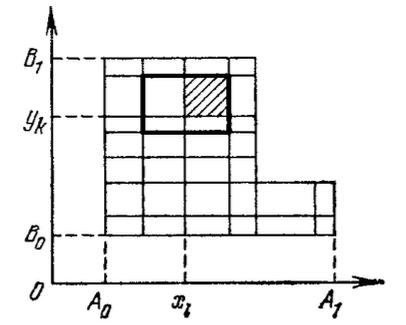
\includegraphics[scale=0.4]{images/12.png}
	\end{center}
	\label{12}
	\caption{Область $\Omega$}
\end{figure}

\[ \left\{
\begin{array}{l}
	- \Delta u + u = f, \qquad f \in L_2 (\Omega) \\
	u|_{\partial \Omega} = g
\end{array}
\right. \]
\[ F(u) = \Int_{\Omega} \left( {\left( \frac{\partial u}{\partial x} \right)}^2 + {\left( \frac{\partial u}{\partial y} \right)}^2 + u^2 - 2uf \right) dx dy \]
\[ H_A = \accentset{\circ}{W}_2^1 (\Omega) \]
\[ \accentset{\circ}{W}_2^{1,h} = \left\{ u^h: u^h \in W_2^{1,h}, \quad u^h = \Sum_{i,j} a_{ij} Q_{ij}, \quad {\| u^h \|}_{\accentset{\circ}{W}_2^{1,h}} = {\| u^h \|}_{W_2^{1,h}}, \quad (x_i, y_j) \in \Omega \right\} \]

\textbf{Теор.} Для любой $u \in W_2^1 (\Omega) \cap C^{(2)}(\Omega)$ существует $u^h \in W_2^{1, h}$ такая, что справедливы оценки \eqref{label}.

\subsection{Построение проекционно сеточной схемы для ОДУ 2-го порядка}

Рассмотрим следующую задачу
\[ \left\{
\begin{array}{ll}
	-\cfrac{d}{dx} \left( p(x) \cfrac{du}{dx} \right) + q(x)u(x) = f(x), \qquad & f \in L_2(a, b) \\
	u(a) = u(b) = 0 \qquad & 0< p_0 \leq p(x) \leq p_1,\ 0 \leq q(x) \leq q_1 \\
\end{array}
\right. \]
\[ Au = f \]
\[ H = L_2 (a, b) \ \Rightarrow \ A \ \text{положительно определен} \ \Rightarrow \ \exists A^{-1} \ \Rightarrow \ \exists! \ \text{решение} \ \eqref{label} \]

Пусть $u(x)$ --- решение \eqref{label}
\[ {\|u\|}_{W_2^2 (\Omega)} \leq c \, {\|f\|}_H \]
\[ H_A = \accentset{\circ}{W}_2^1 (\Omega), \qquad c_0 {\|u\|}_{W_2^1} \leq {\| u \|}_A \leq c_1 {\|u\|}_{W_2^1} \]
\[ F(u) = [u, u] -2 (u, f) \rightarrow \min \quad \text{на} \ \accentset{\circ}{W}_2^1 (\Omega)\]
\[ \varphi_i(x) = \frac{1}{\sqrt{h}} \Biggl\{ ... \]
\[ \accentset{\circ}{W}_2^{1, h} = \left\{ v = \Sum_{i=1}^{N-1} a_i \varphi_i (x) \right\} \subset \accentset{\circ}{W}_2^1 = H_A \]
\[ u^h(x) = \Sum_{i=1}^{N-1} a_i \varphi_i (x) \ \text{--- минимизирует} \ F(v) \ \text{на} \ \accentset{\circ}{W}_2^{1, h} \]

Находим $a_j$ из $\cfrac{\partial F}{\partial a} (u_h) = 0, \quad i=\overline{1, N-1}$

Приходим к системе уравнений
\[ \widehat{A} a = f, \qquad \hat{A} = (A_{ij})\]
\[ A_{ij} = [\varphi_i, \varphi_j] = \Int_{\Omega_{ij}}^{} \left( p \frac{d\varphi_i}{dx}\frac{d \varphi_j}{dx} + q \varphi_i \varphi_j \right) dx \]
\[ a = {(a_1, ... , a_{N-1})}^T, \qquad {f = (f_1, ... , f_{N-1})}^T \]
\[ f_i = \Int_{\Omega_i} f \varphi_i dx \]

Существует единственное решение $ {(a_1, ..., a_{N-1})}^T $, которое однозначно определяет решение $ u^h \leftarrow \underset{v \in \accentset{\circ}{W}_2^{1, h}}{\operatorname{argmin}} \ F(v) $

Отметим, что так как $A_{ij} = 0$ при $|i - j|>1$, то матрица $\widehat{A}$ оказывается трехдиагональной. \\

\textbf{Упр.} Найти $ A_{ij}$ в случае кусочно-постоянных $p$ и $q$ на сетке
\[ p_{i-\frac{1}{2}} = p(x), \quad x \in (x_{i-1}, x_i), \qquad i = \overline{1, N} \]
\[ q_{i-\frac{1}{2}} = ... \]

\newpage
\section{Лекция 13}

\[ \left\{ \begin{array}{l}
	-\cfrac{d}{dx} \left[ p(x) \cfrac{du}{dx}\right] + q(x) u = f \\
	u(a) = u(b) = 0
\end{array} \right. \]
\[ {\|u - u_h\|}_A \leq \|u - v_n\|, \quad \textrm{где} \ v_h = \Sum_{i=1}^{N-1} b_i \varphi_i; \quad \forall v_h \in H_{A}^{(N)} = \accentset{\circ}{W}_2^{1,h} \]
\[ c_0 {\|u\|}_{{W}_2^1} \leq {\|u\|}_A \leq c_1 {\|u\|}_{{W}_2^1} \]
\[ {\|u-u_h\|}_{{W}_2^1} \leq c {\|u - v_h\|}_{{W}^1_2} \]
\[ {\|u-u_h\|}_{{W}_2^1} \leq c \underset{v_h \in H_{A}^{(N)}}{\inf} {\|u - v_h\|}_{{W}^1_2} \]
\[ {\|u-u_h\|}_{{W}_2^1} \leq ch {\|u\|}_{{W}_2^2} \leq ch {\|f\|}_{H=L_2} \]
\[ {\|u-u_h\|}_{{W}_2^1} \leq ch {\|f\|}_{H} \]
\[ {\|u-u_h\|}_{H=L_2} \leq c_2 h {\|f\|}_H \qquad \text{(в силу неравенства Фридрихса)} \]

\[ {[u, v]}_A = (f, v), \quad \forall v \in \accentset{\circ}{W}_2^{1} \]
\[ {[u_h, v_h]}_A = (f, v_h), \quad  \forall v_h \in \accentset{\circ}{W}_2^{1, h} = H_A^{(N)} \]
\[ [u - u_h, v_h] = 0 \quad \forall v_n \in \accentset{\circ}{W}_2^{1, h} \]

Рассмотрим вспомогательную задачу $ A \Phi = F, \ F = u - u_h $

по свойствам A $\exists!$ решение $\Phi$:
\[ {\|\Phi\|}_{W^2_2} \leq c \|F\| = C \|u - u_h\| \]

и $ \Phi $ удовлетворяет: $[\Phi, v] = (F, v) \ \forall v \in \accentset{\circ}{W}_2^{1} $

Рассмотрим $ v = u - u_h $
\begin{multline*}
	(F, v) = (u - u_h, u - u_h) = (A \Phi, u - u_h) = [\Phi, u - u_h] - [u - u_h, \Phi_h] = [\Phi - \Phi_h, u - u_h] \leq \\
	\leq {\|\Phi - \Phi_h\|}_A \cdot {\|u - u_h\|}_A \leq ch \|f\| {\|\Phi - \Phi_h\|}_A \leq \tilde{c} h \|f\| \cdot {\|\Phi - \Phi_h\|}_{W_2^1}
\end{multline*}

Из результатов аппроксимации можно выбрать $ \Phi_h $:
\[ {\|\Phi - \Phi_h\|}_{{W}_2^1} \leq \tilde{c} h \ {\|\Phi\|}_{W^2_2} \]
\[ {\|u-u_h\|}^2 \leq ch {\|f\|} \cdot {\|\Phi- \Phi_h\|}_{{W}_2^1} \leq ch^2 \|f\| \cdot {\|\Phi\|}_{W_2^2} \leq ch^2 \|f\| \cdot \|u - u_h\| \]
\[ \Rightarrow \|u - u_h\| \leq ch^2 \|f\| \cdot \|u - u_h\| \] \\

Рассмотрим задачу с другими граничными условиями
\[ \left\{ \begin{array}{l}
	-\cfrac{d}{dx} \left(p(x) \cfrac{du}{dx}\right) + q(x) u = f(x) \\
	u(a) = 0, \quad \cfrac{du}{dx}(b) = 0
\end{array} \right. \]
\[ u_h = \Sum_{i=1}^N a_i \varphi_i \]

\textbf{Упр.} Проверитть оценки в $ {W'}_2 $

\textbf{Упр.} Найти $ \hat{A} $ при $ h_i = h, i = overline{1, N}, \Phi = 0, P = const $

\subsection{Применение ВП к з. Дирихле для ур-я Лапласа}
\[ \Omega = \{0 < x < a, \ 0 < y < b\} \] 
\[ \left\{ \begin{array}{l}
	- \Delta u = f(x, y) \\
	u|_{\partial \Omega} = 0
\end{array}  \right. \]

\[ A u = - \Delta u \]
\[ D(A) = \{u \in W_2^2(\Omega), \ \ u|_{\partial \omega} = 0 \}, \qquad f \in L_2(\Omega) \]

A --- симметричный положительно определенный
\[ \Rightarrow \forall f \in L_2 \quad \exists! \ n \in \accentset{\circ}{W}_2^1 \cap W_2^2 \]
\[ {\| u \|}_{W_2^2} \leq c \, {\| f \|} \]
\[ H_A = \accentset{\circ}{W}_2^1 (\Omega), \quad {(u, v)}_A = \Int_{\Omega}^{} \left(\frac{\partial u}{\partial x}\frac{\partial v}{\partial x}+\frac{\partial u}{\partial y}\frac{\partial v}{\partial y}\right)d\Omega\]
\[ {[u, v]}_A = (f, v), \quad \forall v \in H_A \]
TODO: картинка + дополнить
\[ \phi_ij = \frac{1}{\sqrt{h_x h_y}} \left\{
\begin{array}{l}
	1 - \left(\cfrac{u}{h_y}-j\right), \quad x_j \leq x \leq x_{i+1} \\
	... \\
	... \\
	\textbf{Упр.}
\end{array} \right. \]
\[ u_h = \Sum_{i=1}^{N_x -1} \Sum_{j=1}^{N_y - 1} a_{ij} \varphi_{ij} (x, y), \qquad H_A^{(N)} = \accentset{\circ}{W}_2^{1, h} \subset H_A = \accentset{\circ}{W}_2^1 \]

$ a_{ij} $ --- решение СЛАУ, \qquad ${[u_h, \varphi_{kl}]}_A = (f, \varphi_{kl}) $
\[ \hat{A} a = f, \qquad \hat{A} = \left( A_{ijkl} \right), \qquad A_{ijkl} = {[\varphi_{ij}, \varphi_{kl}]}_A, \qquad \varphi_{ij} \ \text{--- кусочно линейные} \]
\[ a = \left( a_{1,1}, a_{2,1}, ..., a_{N_x-1,1}, ..., a_{1, N_y-1}, ..., a_{N_x-1, N_y-1} \right), \qquad \textbf{Упр.} \ A_{ijkl} = ? \]

Оценки:
\[ {\|u - u_h\|}_{W_2^1} \leq ch \, \|f\| \]
\[ \|u - u_h\| \leq ch^2 \, \|f\| \]
\[ A = - \frac{d}{dx} (p(x) \frac{du}{dx}) + q(x)u \]

\textbf{Упр.} показать предыдущее выражение

\[ \frac{2a_{ij} - a_{i-1, j} - a_{j+1, i}}{h^2_x} + \frac{2a_{ij} - a_{i, j-1} - a_{i, j+1}}{h^2_y} = f_{ij} = {(f, \varphi_{ij})}_H, \quad i=\overline{1,N_x-1}, \ j=\overline{1,N_y-1} \]
TODO:картинка
\[ \partial  \Omega_h \subset \partial  \Omega \]

$h$ --- $\max$ сторона $ \triangle $

$\theta_0$ --- $\min \angle $
\[ {\|u-u_h\|}_{W_2^1(\Omega)} \leq c \, \frac{h}{sin \theta_0} \|f\| \]
\[ u_h = \Sum_{i=1}^{N} a_i \varphi_i (x, y) \]

\subsection{Подходы к решению неоднородной краевой задачи}

\[ \left\{
\begin{array}{l}
	- \Delta u = f \quad \text{в} \ \Omega \leftarrow \text{выпуклая}, \ \partial \Omega \ \text{гладкая} \\
	u|_{\partial \Omega} = g, \qquad f \in L_2 (\Omega), \ g \in W^{3/2}_2 (\partial \Omega)
\end{array}
\right. \]
\[ c_3 ({\|f\|}_L2 + {\|g\|}_{W_2^{3/2}}) \leq {\|u\|}_{W^2_2(|omega)} \leq c_u() \]

\raisebox{.5pt}{\textcircled{\raisebox{-.9pt} {1}}} Сведение к однородным граничным условиям

Пусть  $\exists \, \Phi \in  D(A): \ \ \Phi=g$ \ на \ $ \partial \Omega $
\[ v = u - \Phi \]
\[ \left\{ \begin{array}{l}
	- \Delta u = \tilde{f} = f + \Delta \Phi \quad \in L_2(\Omega) \\
	u|_{\partial \Omega} = 0,
\end{array} \right. \]
\[ u_h = v_h + \Phi \]
\[ \Phi \in {W}_2^1 (\Omega) \]

\raisebox{.5pt}{\textcircled{\raisebox{-.9pt} {2}}} "Снос" \ граничных условий (с $\partial \Omega$ на $\partial \Omega_h$ )
\[ u_h = \Sum_{i=1}^{\widetilde{N}} a_i \varphi_i (x, y), \qquad \varphi_1, ..., \varphi_N \ \text{--- внутренние узлы}, \ \varphi_{N+1}, ..., \varphi_{\widetilde{N}} \ \text{--- граничные узлы} \]
\[ i = \overline{1, N}: \quad {[u_h, \varphi_i]}_A = (f, \varphi_i) \]
\[ i = \overline{N + 1, \widetilde{N}}: \quad a_i \varphi_i (x_i, y_i) = g(x_i, y_i) \]

\raisebox{.5pt}{\textcircled{\raisebox{-.9pt} {3}}} Метод штрафа

Рассмотрим модифицированную 3 краевую задачу
\[ \left\{
\begin{array}{l}
	- \Delta u_{\varepsilon} = f \quad \text{в} \Omega \\
	u_{\varepsilon} + \varepsilon \cfrac{\partial u}{\partial n} = g \quad \textrm{на} \ \partial \Omega
\end{array}
\right., \qquad \varepsilon > 0 \ \text{мало} \]

Для нее:
\[ {[u, v]}_A = \Int_{\Omega}^{} \left( \frac{\partial u}{\partial x} \frac{\partial v}{\partial x} + \frac{\partial u}{\partial y} \frac{\partial v}{\partial y} \right) d\Omega + \Int_{\partial \Omega}^{} \frac{1}{\varepsilon} u v \, dS \]
\[ u_{\varepsilon, h} = \Sum_{i=1}^{N} a_i \varphi_i(x) \]

$ a_i $ находится из
\[ {[u_h, \varphi_i]}_A = (f, \varphi_i) + \Int_{\partial \Omega} g \varphi_i \, dS \]
\[ {\|u_{\varepsilon} - u_{\varepsilon, h} \|}_{W_2^1 (\Omega)} \leq \frac{ch}{\sin \theta_0} \left( 1 + \frac{h}{\varepsilon} \right) \left({\|f\|}_{L_2} + \frac{1 }{\varepsilon} \| g \|_{W_2^{1/2} \left(\partial \Omega \right)} \right) \]
\[ {\|u_{\varepsilon} - u_{\varepsilon, h} \|}_{L_2 (\Omega)} \leq \frac{ch^2}{\sin^2 \theta_0} {\left( 1 + \frac{h}{\varepsilon} \right)}^2 \left({\|f\|}_{L_2} + \frac{1 }{\varepsilon} \| g \|_{W_2^{1/2} \left(\partial \Omega \right)} \right) \]
\[ {\|u - u_{\varepsilon} \|}_{W_2^1 (\Omega)} \leq c \, \varepsilon \left({\|f\|}_{L_2} + \frac{1 }{\varepsilon} \| g \|_{W_2^{1/2} \left(\partial \Omega \right)} \right) \]

\newpage
\section{Лекция 14}

\subsection{Вариационная постановка задачи на собственные значения \\ симметрично положительного оператора}

\[ A \varphi = \lambda \varphi, \qquad D(A) \subset H \label{14.1} \tag{14.1} \]

A --- симметричный, \qquad $ \lambda $ --- собственные значения, \ $ \lambda \in \mathbb{R} $
\[ \lambda_1 \neq \lambda_2 \quad \text{--- собств. знач.} \ A \quad \Rightarrow \quad (\varphi_1, \varphi_2) = 0\]
\[ (A\varphi, \varphi) = \lambda (\varphi, \varphi) \]
\[ \lambda = \frac{(A\varphi, \varphi)}{(\varphi, \varphi)} \label{eq:14_2} \]

\textbf{Опр.} A ограничен снизу, если $ \forall \varphi \in D(A):$ \\
\[ (A\varphi, \varphi) \geq k(\varphi, \varphi), \quad k \in \mathbb{R} \ \text{(не обязательно $k>0$)} \label{14.2} \tag{14.2} \] \\

Далее A --- ограничено снизу $ \Rightarrow  \cfrac{(A \varphi, \varphi)}{(\varphi, \varphi)} \geq k \Rightarrow \exists \underset{\varphi \in D(A)}{\inf} \cfrac{(A\varphi, \varphi)}{\varphi, \varphi} = d \geq k$
\[ F(\varphi) = \frac{(A \varphi, \varphi)}{(\varphi, \varphi)} \label{14.4} \tag{14.4} \]

\textbf{Теор.} Пусть $ A $ --- симметричн., огр. снизу,  \quad $ d = \underset{\varphi \in D(A)}{\inf} \cfrac{(A \varphi, \varphi)}{(\varphi, \varphi)} $ \\
Если $ \exists \ \varphi_0 \neq 0 \in D(A): \quad F(\varphi_0) = \cfrac{(A \varphi_0, \varphi_0)}{(\varphi_0, \varphi_0)} = d \Rightarrow \exists \min \lambda_1 = d, \quad \varphi_0$ --- собств. функция

\underline{Док-во.}

Пусть $ \eta \in D(A), \quad \forall t \in R, \quad \varphi_0 + t \eta \in D(A) $
\[ \psi(t) = \frac{\bigl( A(\varphi_0 + t \eta), \varphi_0 + t\eta \bigr)}{(\varphi_0 + t \eta, \varphi_0 + t\eta)} = F(\varphi_0 + t \eta) = \frac{t^2(A \eta, \eta) + 2 t \operatorname{Re}(A \varphi_0, \eta) + (A \varphi_0, \varphi_0)}{t^2 (\eta, \eta) + 2t\operatorname{Re}(\varphi_0, \eta) + (\varphi_0, \varphi_0)} \]

Так как $ \varphi_0 = \operatorname{argmin} F(\varphi) \Rightarrow \psi(t) $ в $ t=0 \ \min \Rightarrow \psi'(0) = 0 $
\[ (\varphi_0, \varphi_0): \quad \operatorname{Re} (A \varphi_0 - d \varphi_0, \eta) = 0 \]

Аналогично, заменив $ (\eta) $ на $ (i\eta):$
\[ \operatorname{Im} (A \varphi_0 - d \varphi_0, \eta) = 0 \Rightarrow (A \varphi_0 - d \varphi_0, \eta) = 0 \quad \forall \eta \in D(A) \Rightarrow A \varphi_0 - d \varphi_0 = 0 \Rightarrow A \varphi_0 = d \varphi_0 \]

Следовательно $d$ --- собственное значение, $\varphi_0$ --- собственная функция

Покажем \underline{$\min$}

Пусть $ \lambda_1 $ --- с. зн. $A$
\[ \lambda_1 = \frac{(A \varphi_1, \varphi_1)}{(\varphi_1, \varphi_1)} \geq \frac{(A \varphi_0, \varphi_0)}{(\varphi_0, \varphi_0)} = d \label{14.5} \tag{14.5} \]
\[ \hfill \square \]

\textbf{Теор.} Пусть $ \lambda_1 \leq \lambda_2 \leq ... \leq \lambda_n $ --- собств. знач. симм., огр. снизу A \\
Пусть $ \exists \ \varphi_{n+1} \neq 0 \in D(A): \quad \varphi_{n+1}= \underset{\varphi \in D(A)}{\operatorname{argmin}} \cfrac{(A \varphi, \varphi)}{(\varphi, \varphi)} \quad $ при условии:
\[ (\varphi_{n+1}, \varphi_i) = 0, \quad i=\overline{1,n} \label{14.6} \tag{14.6} \]
\[ \Rightarrow \lambda_{n+1} = \frac{(A \varphi_{n+1}, \varphi_{n+1})}{(\varphi_{n+1}, \varphi_{n+1})} \ \text{--- следующее собств. знач.}, \quad \varphi_{i+1} \ \text{--- собств. функц.} \]
TODO: 7, 8

\underline{Док-во.}
\[ \forall \zeta \in D(A) \]
\[ \eta = \zeta - \Sum_{k=1}^{n} (\zeta, \varphi_k) \varphi_k \]

$ \eta $ удовлетворяет усл \eqref{14.6}

$ t \eta $ удовлетворяет усл \eqref{14.6}

$ \varphi_{n+1} + t \eta \in D(A) $ удовлетворяет усл \eqref{14.6}
\[ \psi(t) = \frac{\bigl(A(\varphi_{n+1}+tn), \varphi_{n+1}+t\eta \bigr)}{(\varphi_{n+1}+t\eta, \varphi_{n+1} + t\eta)} \]

Аналогично \quad $ (A \varphi_{n+1} - \lambda_{n+1} \varphi_{n+1}, \zeta) = 0 \qquad \forall \zeta \in D(A) $ (плотно в $H$)
\[ \Rightarrow A \varphi_{n+1} = \lambda_{n+1} \varphi_{n+1} \]

Пусть $ \exists \lambda' $ --- собств. знач.: \ \ $ \lambda' > \lambda_n, \quad \varphi' $ --- соответствующая собств. функц.
\[ \lambda' = \frac{(A\varphi', \varphi')}{(\varphi', \varphi')} \geq \lambda_{min} = \underset{\varphi \in D_A +  \eqref{14.6}}{\min} \frac{( A \varphi, \varphi )}{(\varphi, \varphi)} \]

$ \lambda_{n+1}$ следующее собственное значение после $ \lambda_n $
\[ \hfill \square \]

\textbf{Теор.}

Пусть оператор опр снизу симм А, содержит тоолько собственные значения  $ \Rightarrow $

$ \Rightarrow \exists min  $ с зн А $ \lambda_0 $ и $ \varphi_0  $ - с ф

$ \frac{(A\varphi_0, \varphi_0)}{(\varphi_0, \varphi_0)} = \lambda_0 $

\[ A \varphi - \lambda B \varphi = 0 \label{eq:14_*} \]

A, B - симметричные, Ф - огр. снизу
В - положительно опр., $  D(A) \subset D(B) \subset H $

Если $ \lambda_0 и \varphi_0 $ - удовлетворяет \ref{eq:14_*} $ \Rightarrow \lambda_0 $ с зн, $ \varphi_0 $ с ф

\[ \lambda_0 = \frac{A \varphi_0, \varphi_0}{(B \varphi_0, \varphi_0)} \]

Теорема

Пусть $ \lambda_k \neq \lambda_m  $ - с зн \ref{eq:14_*}

\[ (B \varphi_k, \varphi_m) = 0; k \neq m  \] - (огр. снизу А не требуется)


Теорема

Пусть $ d - \underset{inf}{\varphi \in D(A)} \frac{(A \varphi, \varphi)}{B \varphi, \varphi} $

Если $ \exists \varphi_0: \frac{(A \varphi_0, \varphi_0)}{(B(\varphi_0, \varphi_0))} = d $

$ \Rightarrow d - min $ - с зн \ref{eq:14_*}, $ \varphi_0 $ - с ф

Теорема

Пусть $ \lambda \leq \lambda \leq ... \leq \lambda $ - с зн \ref{eq:14_*}

$ \varphi_1, ... , \varphi_n $ соответствующие собств функции

Пусть $ \exists \varphi_{n+1} = \underset{argmin}{\varphi \in D(A)}\frac{(A \varphi, \varphi)}{B \varphi, \varphi} $

$ \lambda_n \Rightarrow \lambda_{n+1} = \frac{(A \varphi_{n+1}, \varphi_{n+1})}{(B, \varphi_{n+1}, \varphi_{n+1})} $

\[ (B\varphi, \varphi_k) = 0, k = \overline{1, n} \]

\subsection{Метод Ритца в задаче собственных значений}

Пусть А --- ограниченный снизу оператор

\[ d = \underset{u \in D(A)}{\inf} \frac{(Au, u)}{(u, u)} \label{14.11} \tag{14.11} \] 

По теор. \eqref{по}. Если $ \exists u_0 : \underset{D(A)}{\inf} \cfrac{A \varphi_0, \varphi_0}{\varphi_0, \varphi_0} = d$, то задачу можно свести к
\[ M = \left\{ u: \varphi \in D(A) \cap	 \|\varphi\|=1 \right\} \]
\[ \underset{u \in M}{\inf} (Au, u) \label{14.12} \tag{14.12} \]
\[ (u, u) = 1 \label{14.13} \tag{14.13} \] \\

TODO

Система $ \{ \varphi_n \} \subset D(A)$ полна в H
\[\ \forall u \in D(A) \quad \forall \varepsilon > 0 \quad \exists n \in \mathbb{N} \ \text{и} \ \alpha_1, ... , \alpha_n \in \mathbb{C} \]
\[ \|u - u^*\| < \varepsilon, \qquad u^* = \Sum_{k=1}^{n} \alpha_k \varphi_k \]

Положим
\[ u_n = \Sum_{k=1}^{n} a_k \varphi_k \]

Выберем коэффициенты $a_k$ так, чтобы $u_n$ удовлетворяло \eqref{14.13} и $ (Au_n, u_n) \rightarrow \min $
\[ (A u_n, u_n) = \Sum_{k,m = 1}^{n} (A \varphi_n, \varphi_m) a_k \overline{a_m} \]

удовлетворяющих уравнению
\[ (u_n, u_n) = \Sum_{k, m=1}^{n} (\varphi_k, \varphi_m) a_k \overline{a_m} = 1 \label{14.14} \tag{14.14} \] \\

Метод множителей Лагранжа
\[ \Phi = (A u_n, u_n) - \lambda (u_n, u_n) \]

$ \lambda  $ --- пока неопределенный параметр
\[ \Sum_{k=1}^{m} a_k \left[(A \varphi_k, \varphi_m) - \lambda (\varphi_k, \varphi_m)\right] = 0, \qquad m= \overline{1,n} \label{14.15} \tag{14.15} \]

Однородное СЛАУ относительно $ a_1, ... , a_n $ (одновременно не обр. в ноль) $ \Rightarrow \det (...) = 0 \Rightarrow \ \text{уравнение на} \ \lambda $
\[ \begin{vmatrix}
	(A\varphi_1, \varphi_1) - \lambda (\varphi_1, \varphi_1) & (A\varphi_2, \varphi_1) - \lambda (\varphi_2, \varphi_1) & \dots & (A\varphi_n, \varphi_1) - \lambda (\varphi_n, \varphi_1) \\
	(A\varphi_1, \varphi_2) - \lambda (\varphi_1, \varphi_2) & (A\varphi_2, \varphi_2) - \lambda (\varphi_2, \varphi_2) & \vdots & (A\varphi_n, \varphi_2) - \lambda (\varphi_n, \varphi_2) \\ 
	\vdots & \dots & \ddots & \vdots \\
	(A\varphi_1, \varphi_n) - \lambda (\varphi_1, \varphi_n) & (A\varphi_2, \varphi_n) - \lambda (\varphi_2, \varphi_n) & \dots & (A\varphi_n, \varphi_n) - \lambda (\varphi_n, \varphi_n)
\end{vmatrix}
= 0 \label{14.16} \tag{14.16} \]

Если последовательность $\{ \varphi_n \}$ ортонормирована, то уравнение упрощается
\[ \begin{vmatrix}
	(A\varphi_1, \varphi_1) - \lambda & (A\varphi_2, \varphi_1) & \dots & (A\varphi_n, \varphi_1) \\
	(A\varphi_1, \varphi_2) & (A\varphi_2, \varphi_2) - \lambda  & \dots & (A\varphi_n, \varphi_2)  \\ 
	\vdots & \vdots & \ddots & \vdots \\
	(A\varphi_1, \varphi_n)  & (A\varphi_2, \varphi_n) & \dots & (A\varphi_n, \varphi_n) - \lambda
\end{vmatrix}
= 0 \label{14.17} \tag{14.17} \]

Получаем уравнение $n$-й степени по $\lambda$. Коэффициент при  $ (-1) \lambda^n $ равен определителю матрице Грама для $ \{ \varphi_1, ... \varphi_n \}.$ Отсюда следует, что уравнение имеет ровно $n$ корней \\

Пусть $ \lambda_0 $ --- корень. Пусть $a_k^{(0)}, \quad k=\overline{1,n}$ --- нетривиальное решение. Тогда $ \forall \eta: \, \eta a_k^{(0)}$ также будет решением. Под $a_k^{(0)}$ теперь будем понимать $\eta a_k^{(0)}$. Подставив $\eta a_k^{(0)}$ в \eqref{14.14} найдем $\eta$. Подставив в \eqref{14.15} $\lambda = \lambda_0$ и $a_k = a_k^{(0)}$, умножим на $\overline{a_m^{(0)}}$ и просуммируем $\Sum_m (...)$, получим:
\[ \underbrace{\Sum_{k,m=1}^{n} a_k^{(0)} \overline{a_m^{(0)}} (A \varphi_k, \varphi_m)}_{= \left(Au_n^{(0)}, u_n^{(0)}\right)} = \lambda_0 \underbrace{\Sum_{k,m=1}^{n} (\varphi_k, \varphi_m) a_k^{(0)} \overline{a_m^{(0)}}}_{=1 \ \eqref{14.14}} \]
\[ \lambda_0 = \left(Au_n^{(0)}, u_n^{(0)}\right), \qquad u_n^{(0)} = \Sum_{k=1}^n a_k^{(0)} \varphi_k \]
\[ \underset{M}{\min} (Au, u) = \min \, \text{из $\lambda$ корней} \]



\end{document}